\chapter{Le prototype de calorimètre à lecture semi-digitale}
\label{chap.sdhcal}
Dans ce chapitre le prototype de calorimètre à lecture semi-digitale qui a été construit au sein de l’institut de physiques nucléaire de Lyon en 2011 sera décrit. Ce prototype a été testé lors de plusieurs campagnes de test en faisceau au CERN. Pendant ces tests, le prototype a été exposé à un flux de particules tel que des pions, des protons, des muons et des électrons. Nous détaillerons les différents méthodes utilisées pour reconstruire l’énergie des hadrons incidents. 
\minitoc
\newpage

%%%%%%%%%%%%%%%%%%%%%%%%%%%%%%%%%%%%%%%%%%%%%%%

\section{Les gerbes hadroniques}
Lorsqu'un hadron de haute énergie traverse un matériau dense, il interagit avec les noyaux de celui-ci. Cette interaction produit généralement plusieurs particules secondaires qui vont à leur tour interagir avec le milieu et créer d'autres particules. L'ensemble de ces processus constitue une gerbe hadronique.  La gerbe hadronique prend fin lorsque l'énergie des particules filles n'est plus suffisante pour créer des hadrons. Cependant des processus de basse énergie vont continuer jusqu'à l'arrêt ou l'absorption des particules filles. Ce phénomène de gerbe hadronique s'observe dans les expérience de physique de particules où les hadrons créé voyagent jusqu'aux calorimètres. Ils induisent alors ces cascades de particules. L'énergie déposée et mesurée dans les calorimètres permet alors de retrouver l'énergie de la particule incidente. Ce phénomène s'observe aussi dans l'atmosphère lorsqu'un rayon cosmique interagit dans l'atmosphère. Ces rayons cosmiques peuvent être des gammas, des protons, des noyaux d'hélium, des électrons... Les rayons cosmiques sont principalement générés à l'extérieur du système solaire et pourraient avoir comme origine des noyaux actifs de galaxie, l'explosion de supernovas ou des trous noirs. La figure~\ref{fig:cosmicShowerScheme} montre un schéma de développement d'une gerbe hadronique induite par un proton cosmique.
\begin{figure}[!h]
  \begin{center}
    \includegraphics[width=.7\textwidth]{SDHCAL/figs/cosmicShower.jpg}
    \caption{Schéma du développement d'une gerbe hadronique induite par un proton cosmique.}
    \label{fig:cosmicShowerScheme}
  \end{center}
\end{figure}
Ce schéma illustre le nombre important de variétés de particules secondaire pouvant être générer. On peut distinguer deux composantes dans les gerbes hadroniques: une partie électromagnétique et et une non-électromagnétique.\\

La fraction électromagnétique est composée d'électrons et de photons, provenant souvent de la désintégration des mésons neutres $\pi^{0}$ et $\eta$. Les processus mis en jeu dans cette composante sont les suivants:  
\begin{itemize}
\item Le rayonnement Bremsstralung: $e^-~+~noyau~\rightarrow~e^-~+~\gamma$ 
\item La production de paire (pour des photons d'énergie supérieure à $1022\ keV$): $\gamma~+~noyau~\rightarrow~e^+e^-$  
\item L'annihilation: $e^+~+~atome~\rightarrow~2\gamma~+~ion$
\item L'effet compton: $\gamma~+~atome~\rightarrow~\gamma~+~e^-~+~ion$
\item L'effet photoélectrique (pour des photons de faible énergie): $\gamma~+~atome~\rightarrow~e^-~+~ion$ 
\end{itemize}
La fraction non électromagnétique est plus complexe. En effet, en plus de l’ionisation par les particules chargées, des processus d'interaction faible et forte sont mis en jeu. Des interactions inélastiques des hadrons avec les noyaux du milieu produisent des particules secondaires. Les noyaux sont souvent laissés dans des états excités après ces interactions. Ils retrouvent un état fondamental via des processus de désintégrations et de fragmentations nucléaires. De plus, plusieurs effets induisent des difficultés supplémentaires ou des erreurs pour l'analyse des gerbes hadroniques. D'une part, une fraction de l'énergie hadronique est invisible, à cause de la capture stable de protons ou de neutrons par des noyaux. 
D'autre part, une autre fraction de l'énergie hadronique est détectée avec du retard. En effet, les processus d'interaction faible et forte peuvent entraîner l'émission de neutrons qui ont besoin de se thermaliser pour se lier à un noyau. Ces phénomènes peuvent exciter des noyaux avec un retard par rapport au développement de la gerbe hadronique car la thermalisation des neutrons est un phénomène lent. La désintégration tardive de ces noyaux, peut engendrer une perte d'information pour l’événement ou même du bruit pour les événements suivants. Enfin les muons et les neutrinos émis pendant le développement de la cascade peuvent s'échapper du détecteur. La fraction d'énergie manquante entraînera des difficultés pour la mesure de l'énergie de la particule incidente et dégradera la résolution en énergie du détecteur.
\begin{figure}[!h]
  \begin{center}
    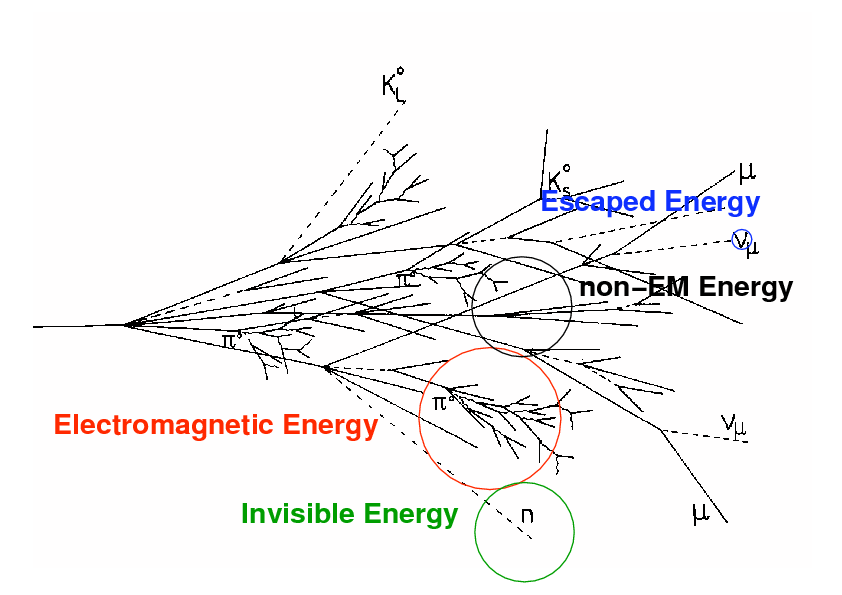
\includegraphics[width=.8\textwidth]{SDHCAL/figs/had-shower.png}
    \caption{Schéma du développement d'une gerbe hadronique.}
    \label{fig:showerScheme}
  \end{center}
\end{figure}
La figure~\ref{fig:showerScheme} montre un schéma de gerbe hadronique. Les différentes composantes de la cascade sont sont mis en évidence.

%%blabla sur la longuer d'interaction

%%%%%%%%%%%%%%%%%%%%%%%%%%%%%%%%%%%%%%%%%%%%%%%

\section{Le SDHCAL}
Le calorimètre hadronique à lecture semi-digitale est un concept de calorimètre à échantillonnage développé au sein de la collaboration CALICE. La partie active est composée de chambres à plaques résistives de verre (GRPC). Un prototype de calorimètre à lecture semi-digitale a été construit en 2011 à l’institut de physique nucléaire de Lyon. Les principaux objectifs de ce prototype étaient de montrer qu'un calorimètre gazeux ultra-granulaire peux réaliser des mesures précises de l'énergie de hadrons et de valider l'intérêt de ce type de détecteur pour l'application d'algorithmes de suivi de particules (Paricule Flow Algorithm PFA). Il est composé de 48 chambres à plaques résistives de verre  de 1 $m^2$, insérées dans des cassette en acier de 0.25 $cm$ d'épaisseur qui participe à l'absorbeur. Ces cassettes sont insérées dans une structure autoporteuse en acier construit dans le laboratoire CIEMAT en Espagne. Les cassettes sont alors séparées par des plaques en acier de 1.5 $cm$ d'épaisseur. Ainsi les GRPC du prototypes sont séparées par 2 $cm$ d'acier. La taille du prototype est $1\times1\times1.3~m^3$ et sa profondeur totale correspond à 6$\lambda_I$ ($\lambda_I\simeq20.4~cm$ pour les pions dans le fer). La figure~\ref{fig:proto} est une photographie du prototype sur la ligne de faisceau H6 du SPS (Super Proton Syncrotron) au CERN.
\begin{figure}[!h]
  \begin{center}
    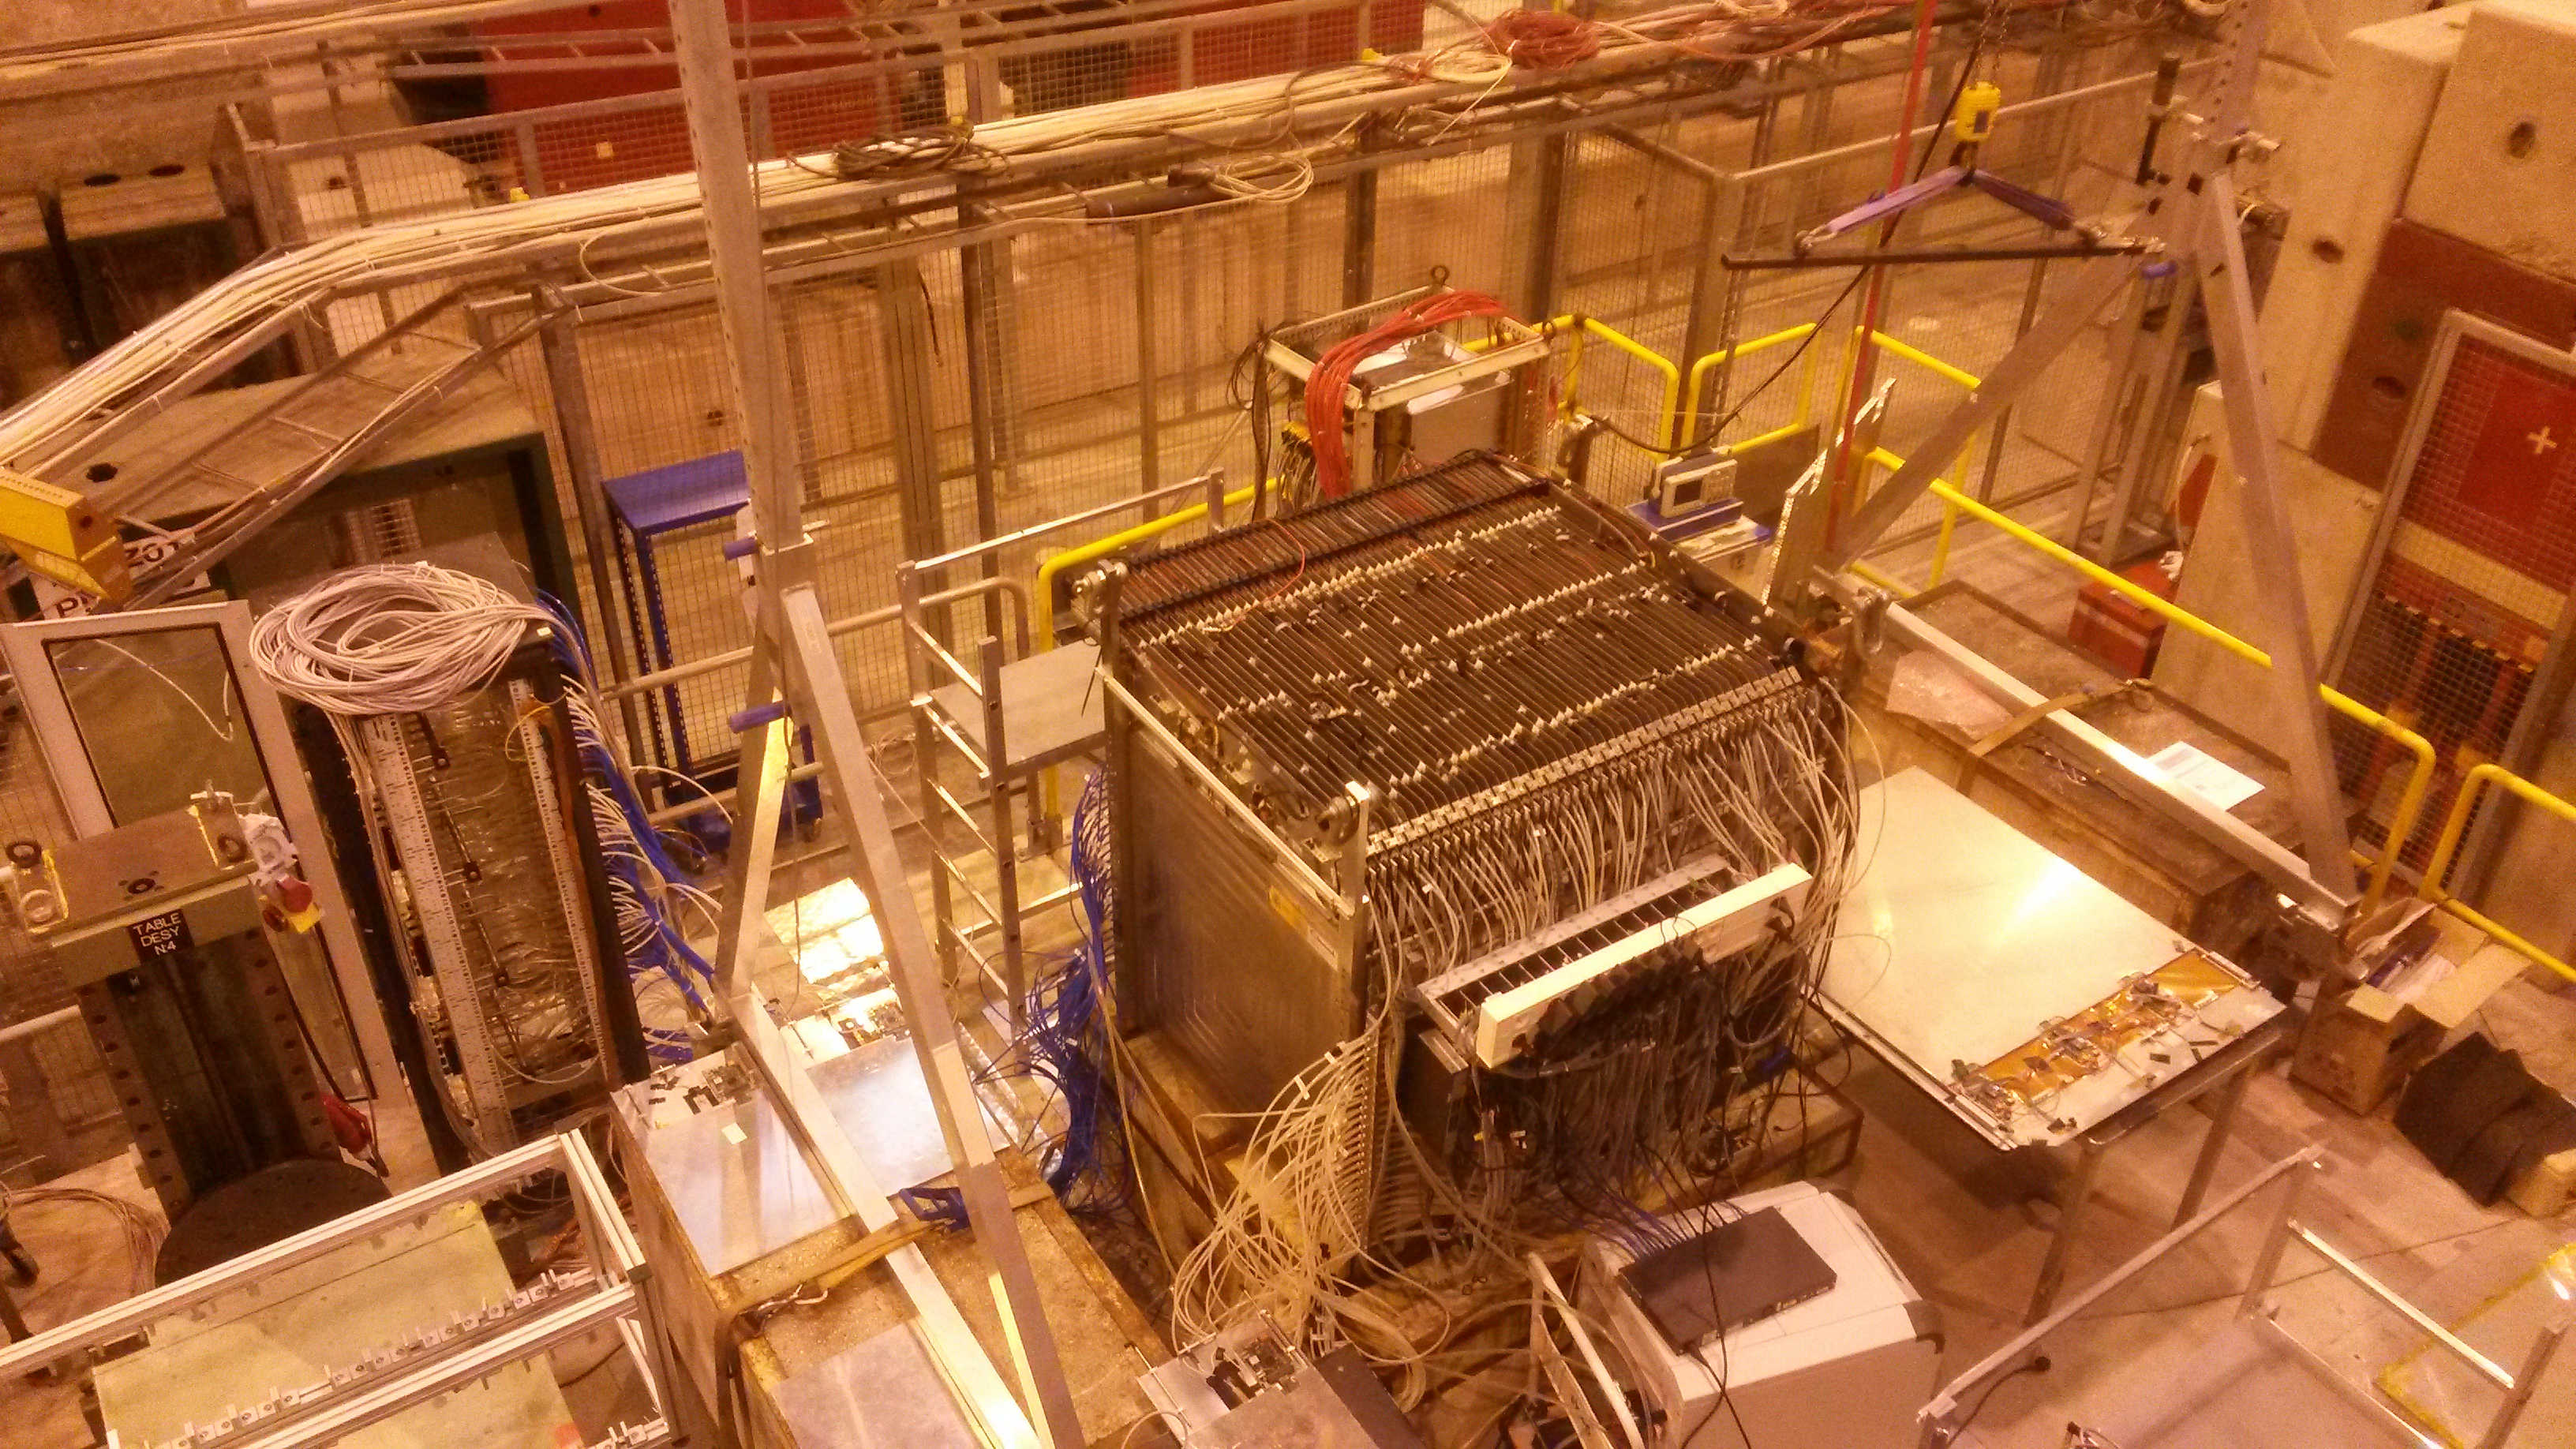
\includegraphics[width=.8\textwidth]{SDHCAL/figs/proto.jpg}
    \caption{Le prototype du calorimètre à lecture semi-digitale sur la ligne de faiceau H6 du CERN.}
    \label{fig:proto}
  \end{center}
\end{figure}
%
Contrairement à la majorité des calorimètres, le SDHCAL n'a pas été optimisé pour obtenir la meilleurs résolution en énergie possible. En effet, la résolution en énergie d'un calorimètre est souvent étroitement liée à sa fraction d'échantillonage. Cette fraction correspond au rapport entre l'énergie déposée par la cascade dans la partie active du détecteur (le gaz des GRPCs pour notre détecteur) et l'énergie totale déposée. Cette fraction est presque nulle pour le SDHCAL alors qu'elle est peut être égale à 1 dans le cas de calorimètres homogènes où l'absorbeur et le milieu actif sont confondus (exemple: le calorimètre électromagnétique de CMS). Cependant, les deux principales particularités de ce détecteur sont sa granularité et son mode de lecture semi-digital. Chaque GRPC a une segmentation transverse de 1 $cm^2$. Le mode semi-digital signifie que trois seuils sont appliqués sur la charge déposée dans les cellules de lecture des GRPCs. Ces seuils permettent non pas de mesurer l'energie déposée dans le détecteur mais d'avoir une idée du nombre de particules secondaires créée dans la cascade. Les informations sur les seuils et sur la geométrie de la cascade seront ensuite utilisées pour mesurer l'énergie des particules incidentes. La figure~\ref{fig:shower80} montre le développement d'une gerbe hadronique de 80 GeV dans les plans (XZ) et (YZ) enregistrée par le prototype du SDHCAL sur la ligne H6 du SPS au CERN.
\begin{figure}[!h]
  \begin{center}
    \includegraphics[width=.8\textwidth]{SDHCAL/figs/pion80GeV.pdf}
    \caption{Exemple de gerbe hadronique induite par un pion de 80 GeV dans le prototype SDHCAL. Les couleurs correspondent aux différents seuils de lecture.}
    \label{fig:shower80}
  \end{center}
\end{figure}
Les points verts, bleus et rouges correspondent aux coups enregistrés avec les seuils 1, 2 et 3 respectivement. On constate que les coups associés aux deux seuils supérieurs sont majoritairement situés au centre de la cascade où la densité de particules secondaire est théoriquement la plus importante. Nous verrons par la suite comment les informations relatives aux trois seuils nous aident à améliorer les performances du détecteur. De plus, sur la figure~\ref{fig:shower80} on distingue des branches où aucune nouvelle particule secondaire n'est crée. La reconstruction de ces branches ou traces sera aussi utilisée lors de la mesure de l'énergie des particules incidentes.
%%%%%%%%%%%%%%%%%%%%%%%%%%%%%%%%%%%%%%%%%%%%%%%

\section{Les chambres à plaques résistives de verre}
Nous allons maintenant décrire les chambres à plaques résistives de verre utilisées comme partie active du SDHCAL. 
\subsection{Géométrie d'une GRPC}
Une chambre à plaque résistive est un détecteur gazeux composé de deux électrodes faites avec un matériau dont la résistivité varie entre $10^7$ et $10^{12}~\Omega cm$. Ces électrodes sont séparées par une fine couche de gaz allant jusqu'à quelques millimètres. Une peinture condutrice sur la face externe de ces électrodes permet d'appliquer une haute tension. Le gaz est souvent une mélange fait base de tétrafluoroéthilène et de SF6. Ainsi lorsque qu'une particule chargée traverse la couche de gaz, quelques molécules de gaz sont ionisés. Les électrons et les ions ainsi créés, sont accélérés par le fort champ électrique généré par la haute tension puis ionisent à leur tour d'autres molécules. Une cascade électronique est alors créée puis le signal est lu par induction. Ces détecteurs permettent d'obtenir une bonne résolution spatial et d'une résolution temporelle de l'ordre de 1 $ns$ avec une épaisseur de la couche de gaz de 2 $mm$~\cite{riegler}. Il est aussi possible d'obtenir de meilleurs résolution temporelle avec des couches de gaz plus fine. Les RPCs sont utilisés comme détecteur de muons dans les expériences ATLAS~\cite{atlas} et CMS~\cite{cms}. Pour ces deux expériences, les électrodes sont en bakélite. Ce matériaux a une résistivité volumique de l'ordre de $\rho\simeq10^{10}\Omega cm$. La résistivité volumique des électrodes est un paramètres très important pour les RPCs. En effet, les charges issues de la cascade électroniques déposées sur les électrodes écrantent le champ électrique et celui chute localement dans la couche de gaz. Ainsi le détecteur sera aveugle pendant un certain temps la région de la cascade. La résistivité du bakélité lui permet d'être très efficace sous un flux de particules allant jusqu'à quelques $kHz/cm^2$. \textcolor{red}{Cependant pour des raisons qu'Imad m'expliquera on ne peut pas utilisé le bakélite.} Pour le SDHCAL, le verre a été choisi pour les électrodes. La résistivité volumique du verre est $\rho=10^{12}\Omega cm$. La figure~\ref{fig:grpc} présente un schéma des GRPCs utilisées pour le prototype du SDHCAL. 
\begin{figure}[!h]
  \begin{center}
    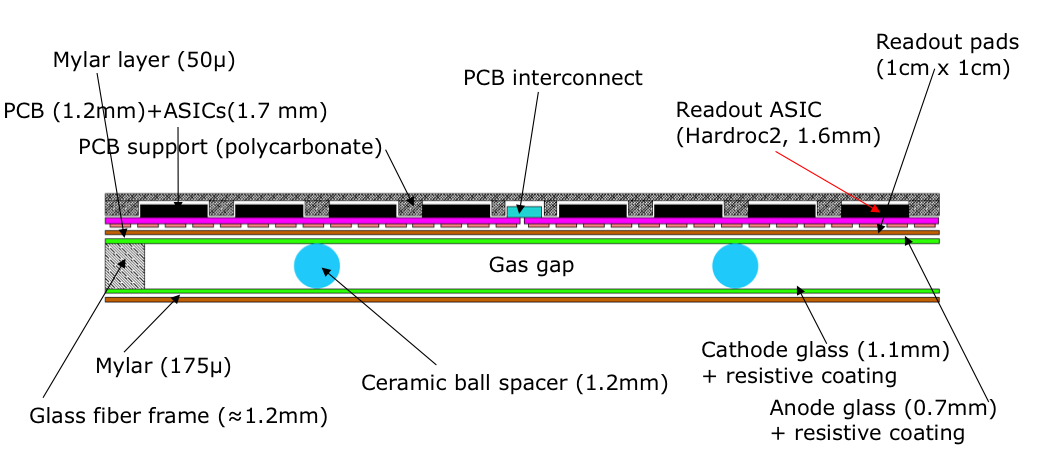
\includegraphics[width=.8\textwidth]{SDHCAL/figs/GRPC-K7.png}
    \caption{Schéma d'une GRPC.}
    \label{fig:grpc}
  \end{center}
\end{figure}
L'anode et la cathode ont des épaisseurs de 0.7 et 1.1 $mm$ respectivement. La peinture appliquée sur ces électrodes est une peinture bi-composant à base de graphite colloïdal. Les électrodes sont séparés par une couche de gaz de 1.2 $mm$ d'épaisseur. Cette épaisseur est garantit par des billes en ceramique de 1.2 $mm$ de diamètre collées sur les électrodes. Des carreau de cuivre capacitifs de 1 $cm^2$ (figure~\ref{fig:carreaux}) utilisés pour collecter la charge sont directement imprimer de l'autre coté du circuit de lecture. Chaque GRPC contient 9216 carreaux de cuivre, ce qui conduit à plus de de 440000 canaux de lecture pour le prototype.
\begin{figure}[!h]
  \begin{center}
    \includegraphics[width=.8\textwidth]{SDHCAL/figs/PADs.png}
    \caption{Les carreaux de cuivres capacitifs de 1 $cm^2$ imprimés de l'autre coté du circuit de lecture d'une petite chambre utilisée pendant le développement du détecteur.}
    \label{fig:carreaux}
  \end{center}
\end{figure}
Une feuille de Mylar de 50 $\mu m$ est déposée entre l'anode et les carreaux de cuivre pour isoler ces derniers. Le circuit de imprimé lecture PCB (Printed Circuit Board) est composé de 6 ASUs (Active Sensor Unit) soudés entre eux. Sur chaque ASU, 24 ASICs (Application Specifique Integrated Circuit) HARDROC2~\cite{omega} sont déposés. Chacun de ces ASICs sont reliés à 64 carreaux de cuivre. 
\begin{figure}[!h]
  \begin{center}
    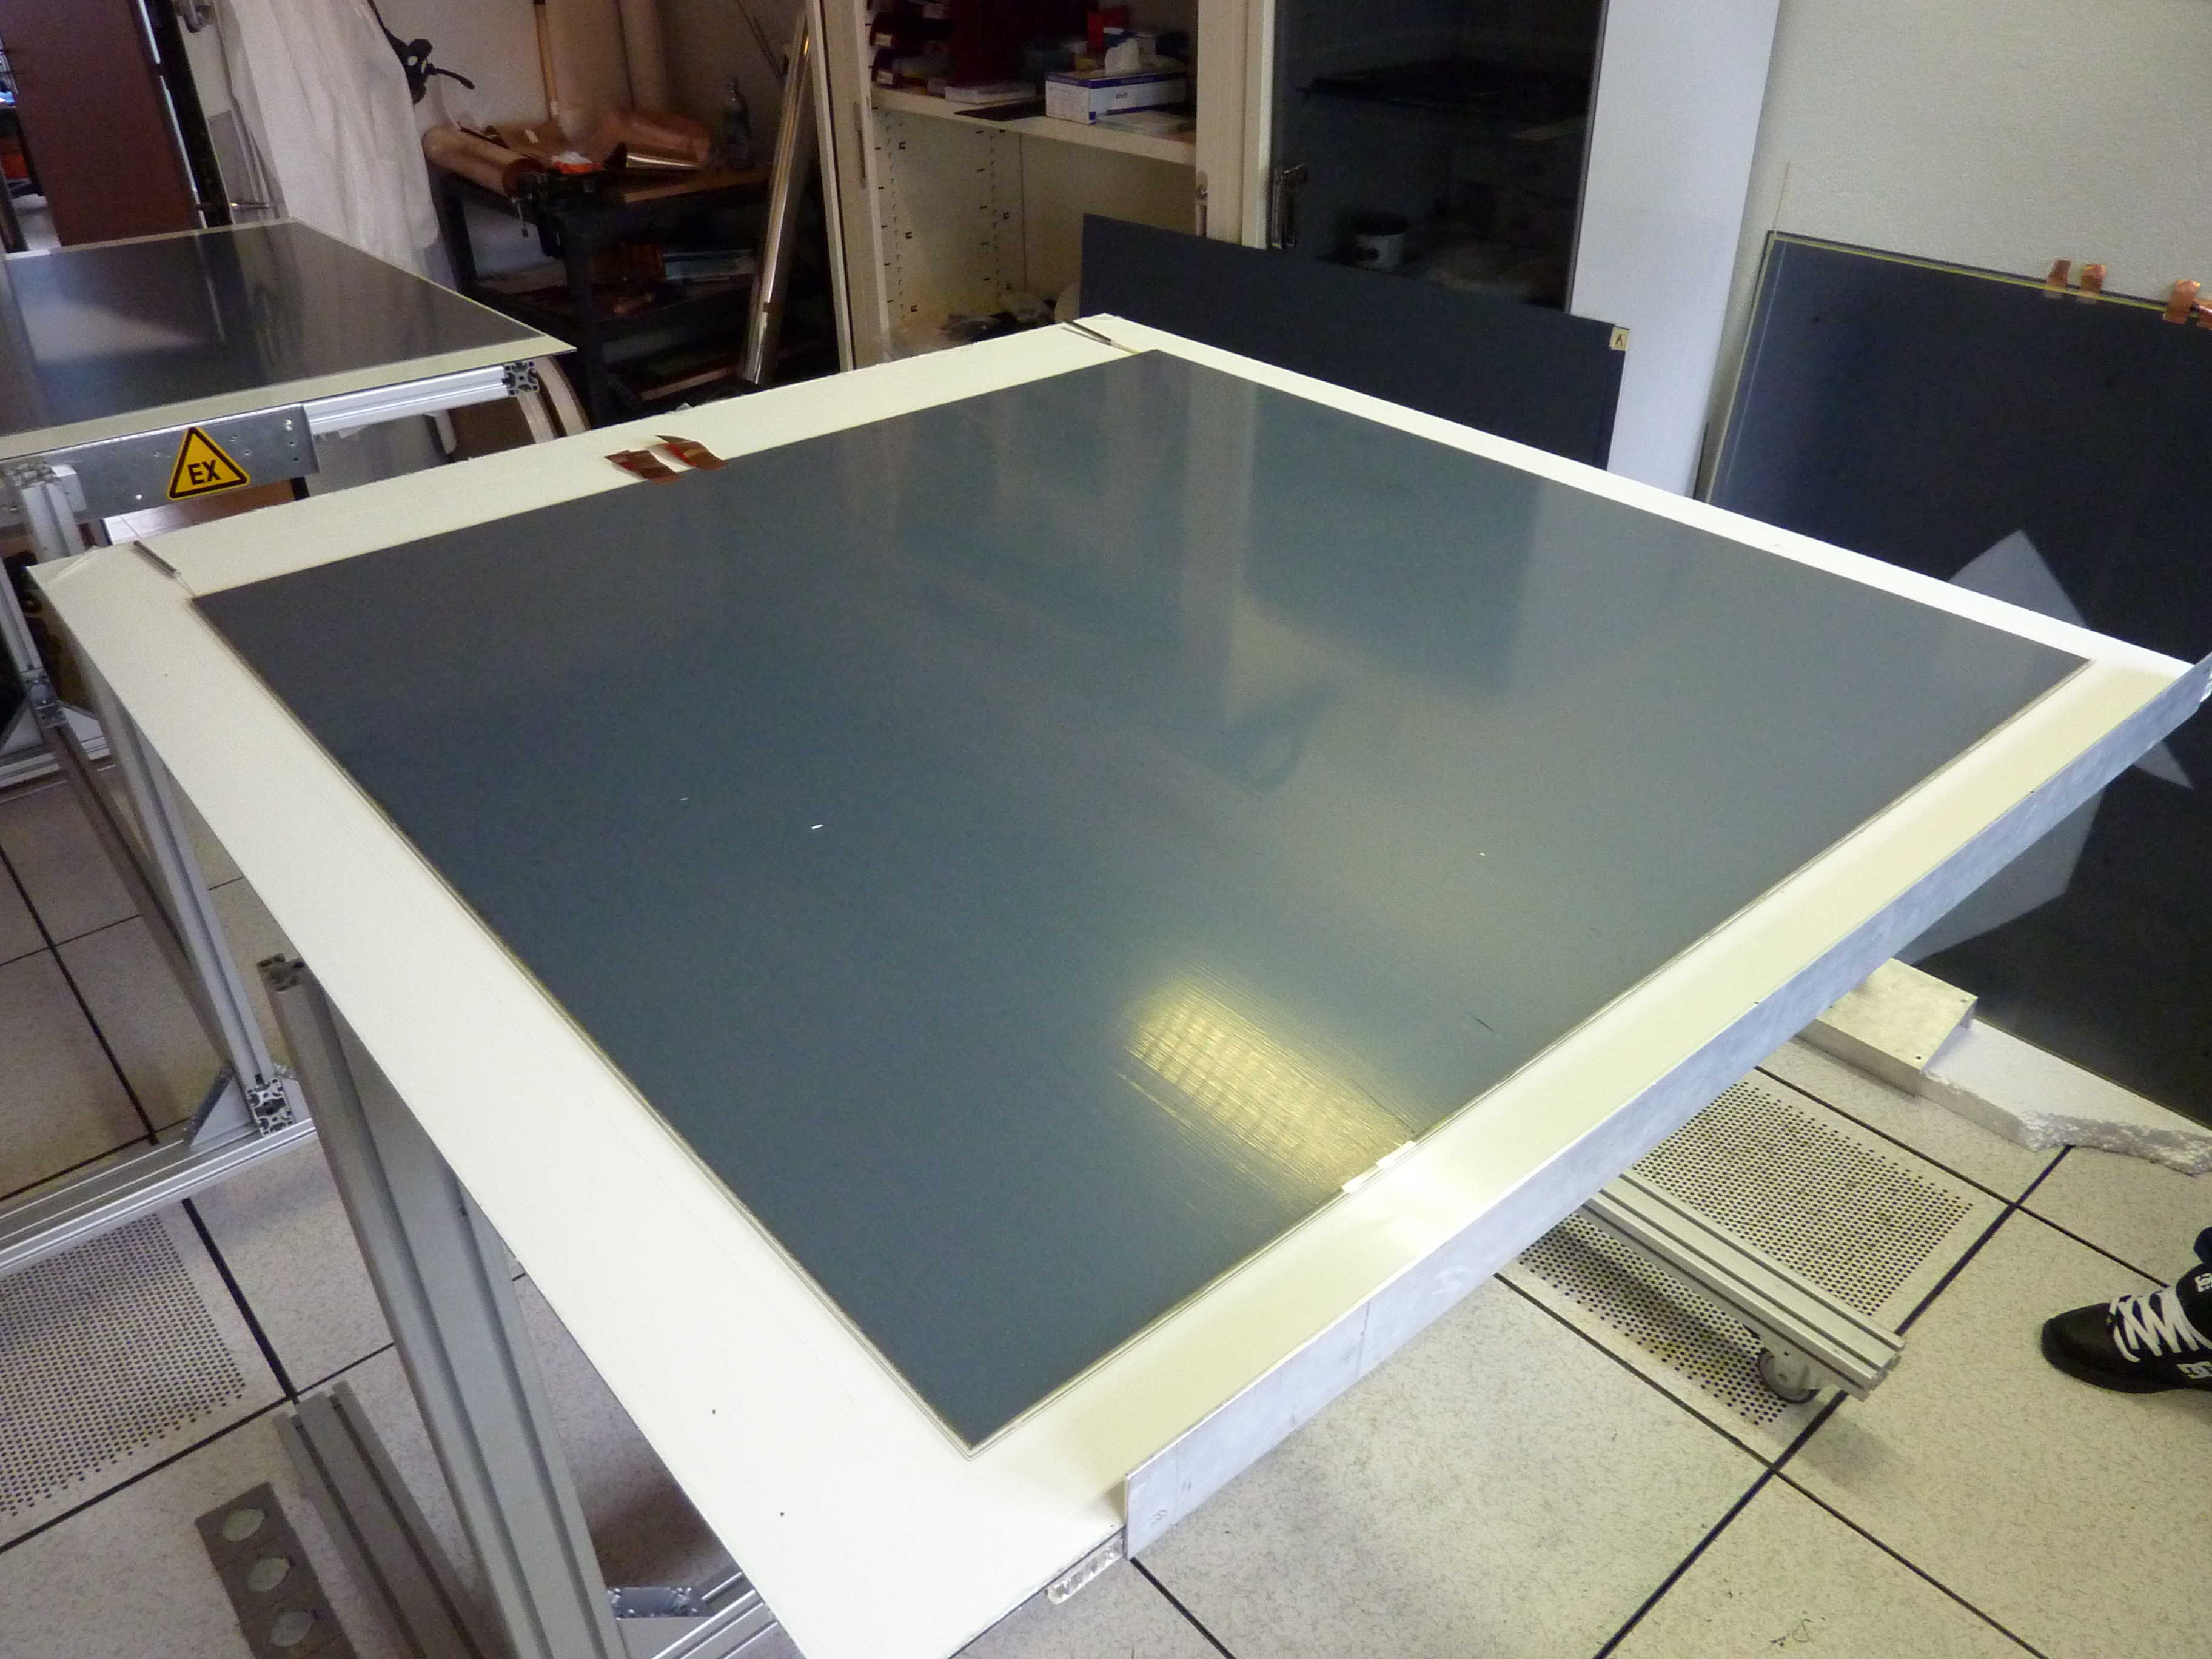
\includegraphics[width=.47\textwidth]{SDHCAL/figs/aLayer.jpg}
    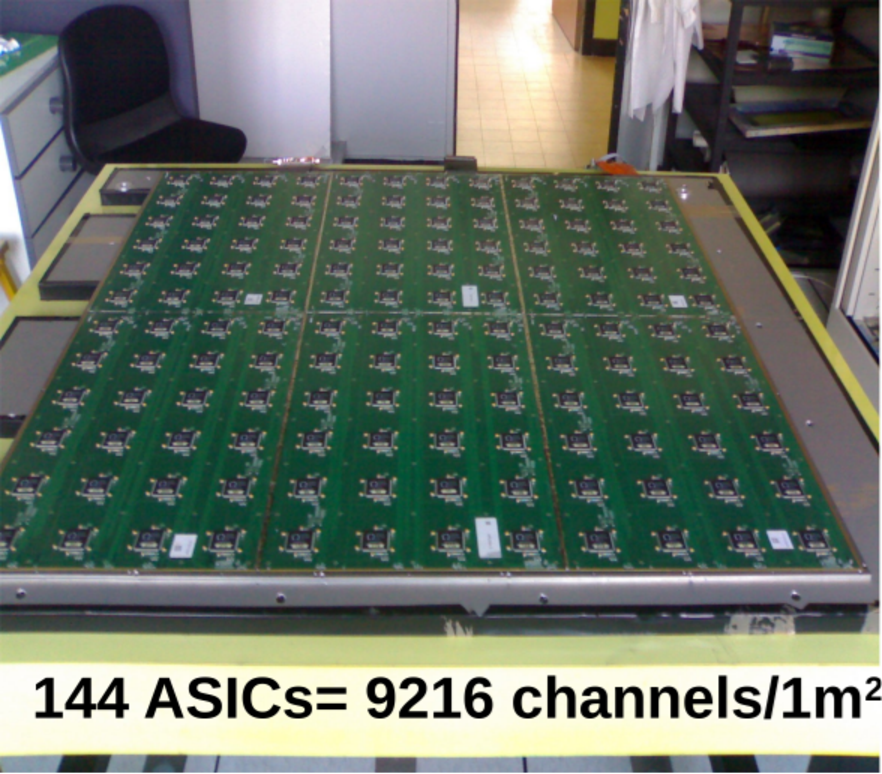
\includegraphics[width=.4\textwidth]{SDHCAL/figs/layer_electronic2.pdf}
    \caption{Photo de plan de rpc et d'un plan d'électronique.}
    \label{fig:layer}
  \end{center}
\end{figure}

\subsection{Le fonctionement d'une GRPC}
%hv, mélange de gaz, avalanche courbe d'efficacité + plateau

\subsection{Alimentation pulsée}
%réduction de la consommation + blabla ILC + spill SPS

\subsection{Le réglage des seuils}
% ok

\subsection{Correction des gains}
% plot carte de gain, temps d'acqisition avant/après

%%%%%%%%%%%%%%%%%%%%%%%%%%%%%%%%%%%%%%%%%%%%%%%

\section{Reconstruction de l'énergie dans le SDHCAL}

\subsection{Reconstruction des évenements}
\label{sec.trivent}
\begin{figure}[!h]
  \begin{center}
    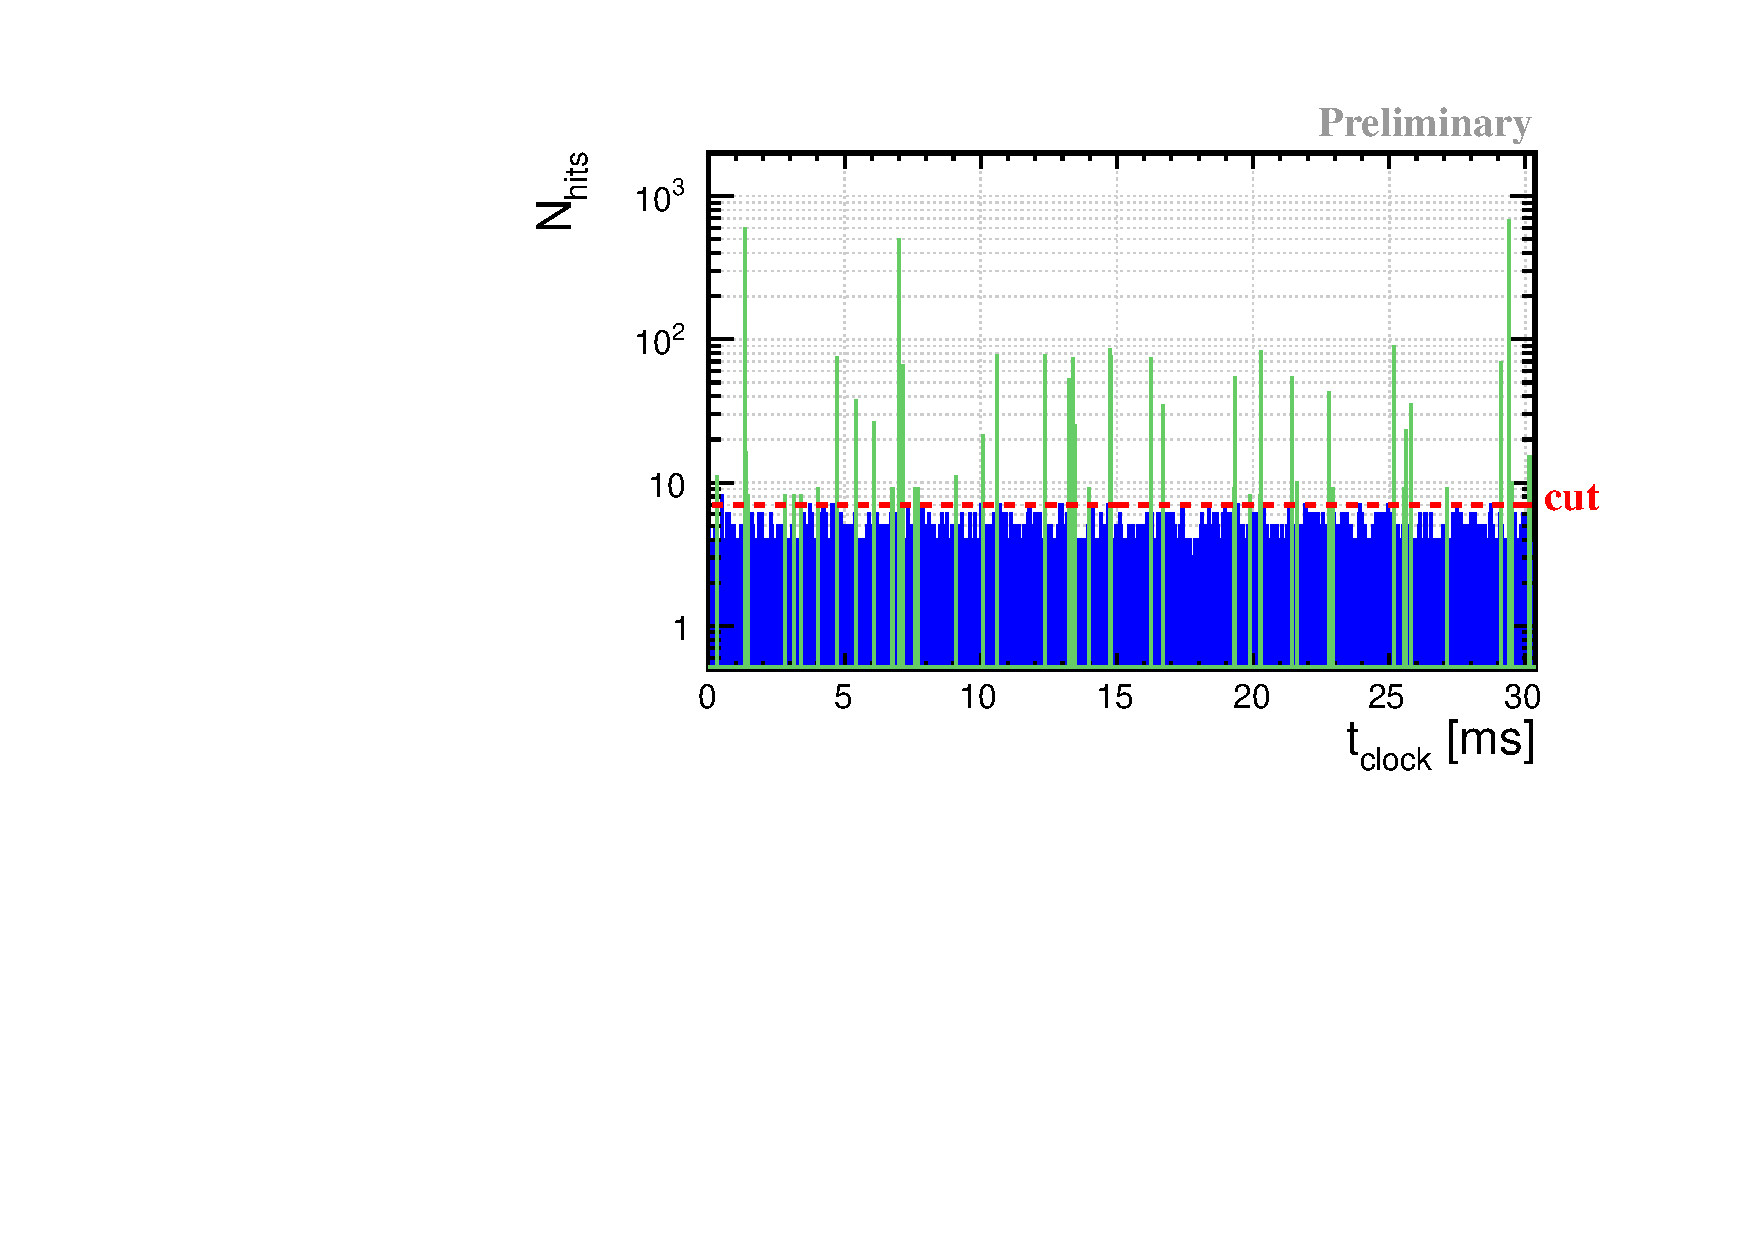
\includegraphics[width=.8\textwidth]{SDHCAL/figs/time_spectrum.pdf}
    \caption{Histogram des temps dans un trigger.}
    \label{fig:time_spectrum}
  \end{center}
\end{figure}

\subsection{Performance du SDHCAL}
\label{sec.muons}
\begin{figure}[!h]
  \begin{center}
    \includegraphics[width=.45\textwidth]{SDHCAL/figs/eff_layer_august_fit.pdf}
    \includegraphics[width=.45\textwidth]{SDHCAL/figs/mul_layer_august_fit.pdf}
    \caption{Selections des pions.}
    \label{fig:pion_selection}
  \end{center}
\end{figure}

\subsection{Sélection des gerbes hadroniques}
\label{sec.shower_selection}
\begin{figure}[!h]
  \begin{center}
    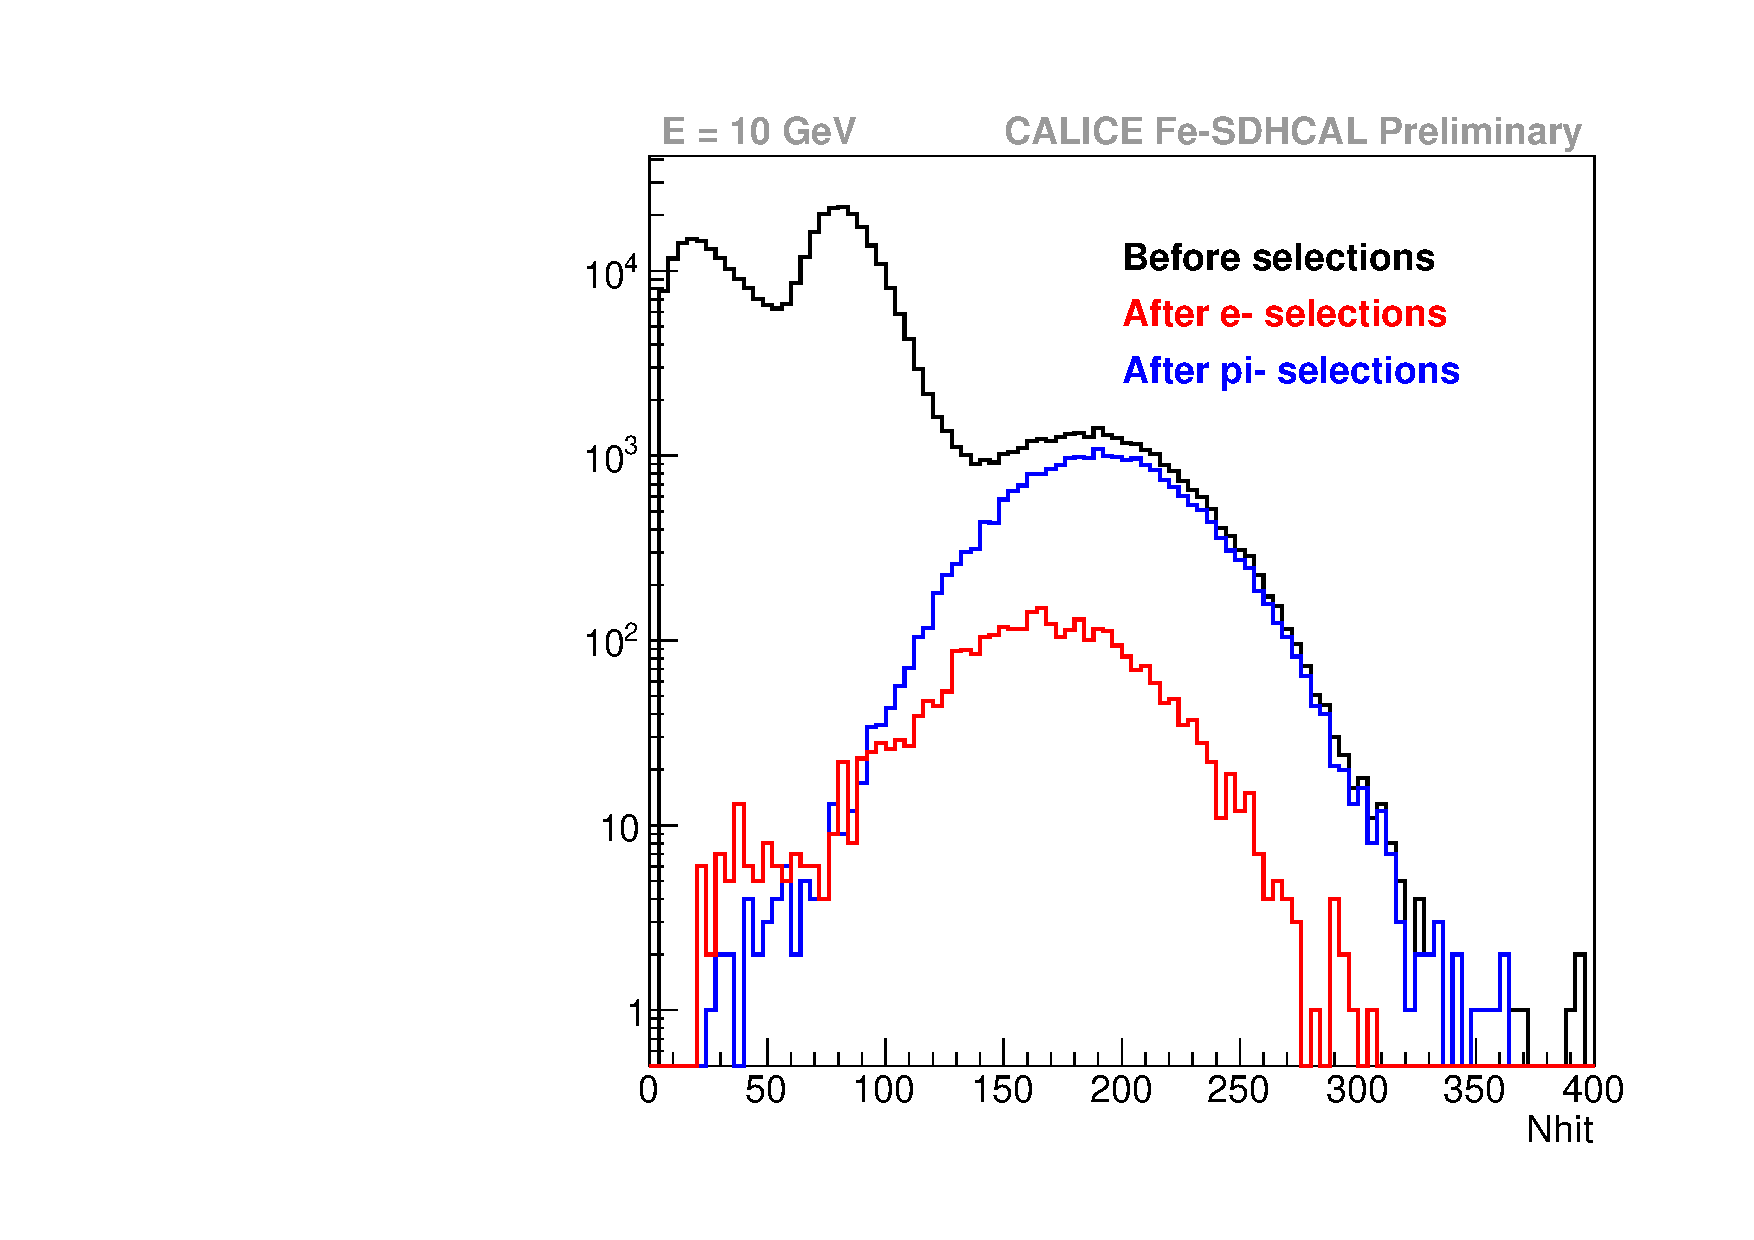
\includegraphics[width=.45\textwidth]{SDHCAL/figs/selection715693.pdf}
    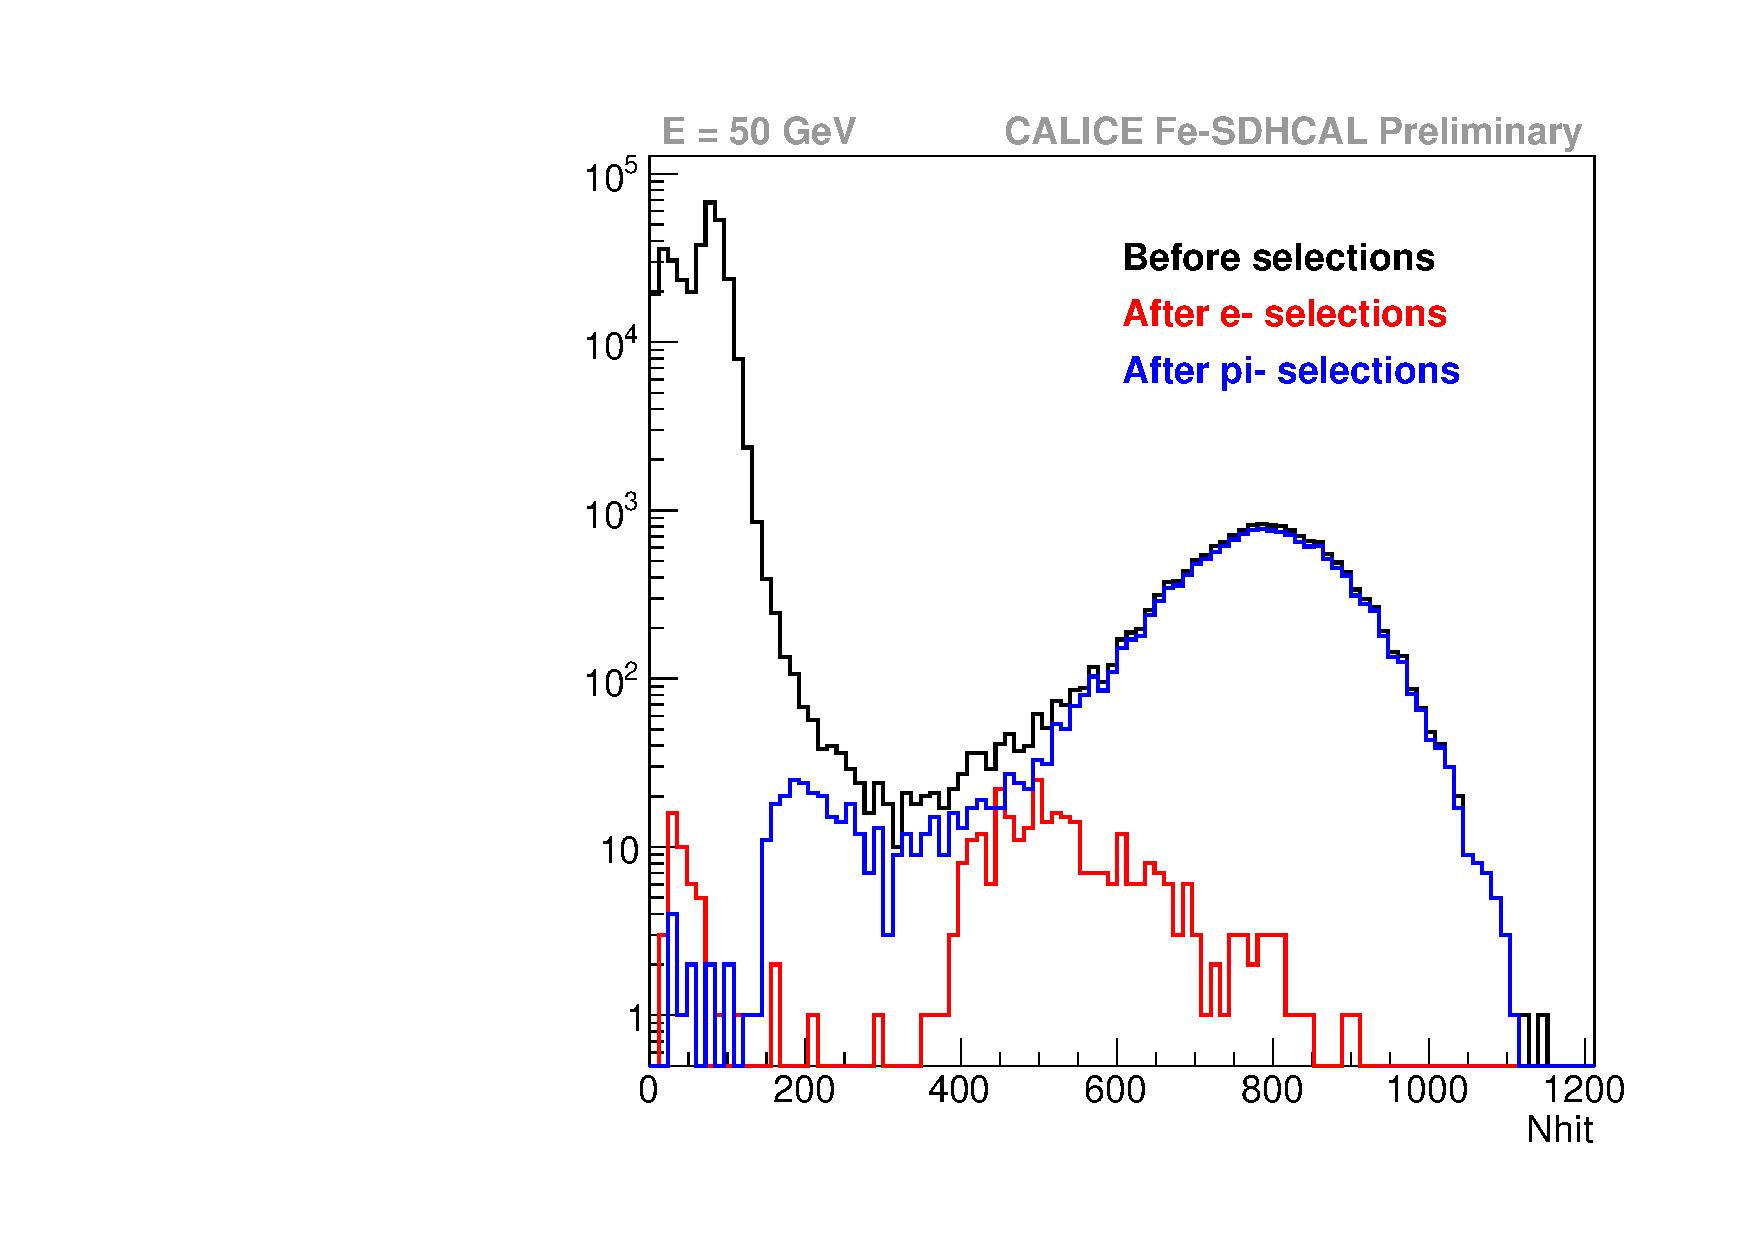
\includegraphics[width=.45\textwidth]{SDHCAL/figs/selection715751.pdf}
    \caption{Selections des pions.}
    \label{fig:pion_selection}
  \end{center}
\end{figure}

\subsection{Calibration en fonction du temps}
\label{sec.timeCalib}
\begin{figure}[!h]
  \begin{center}
    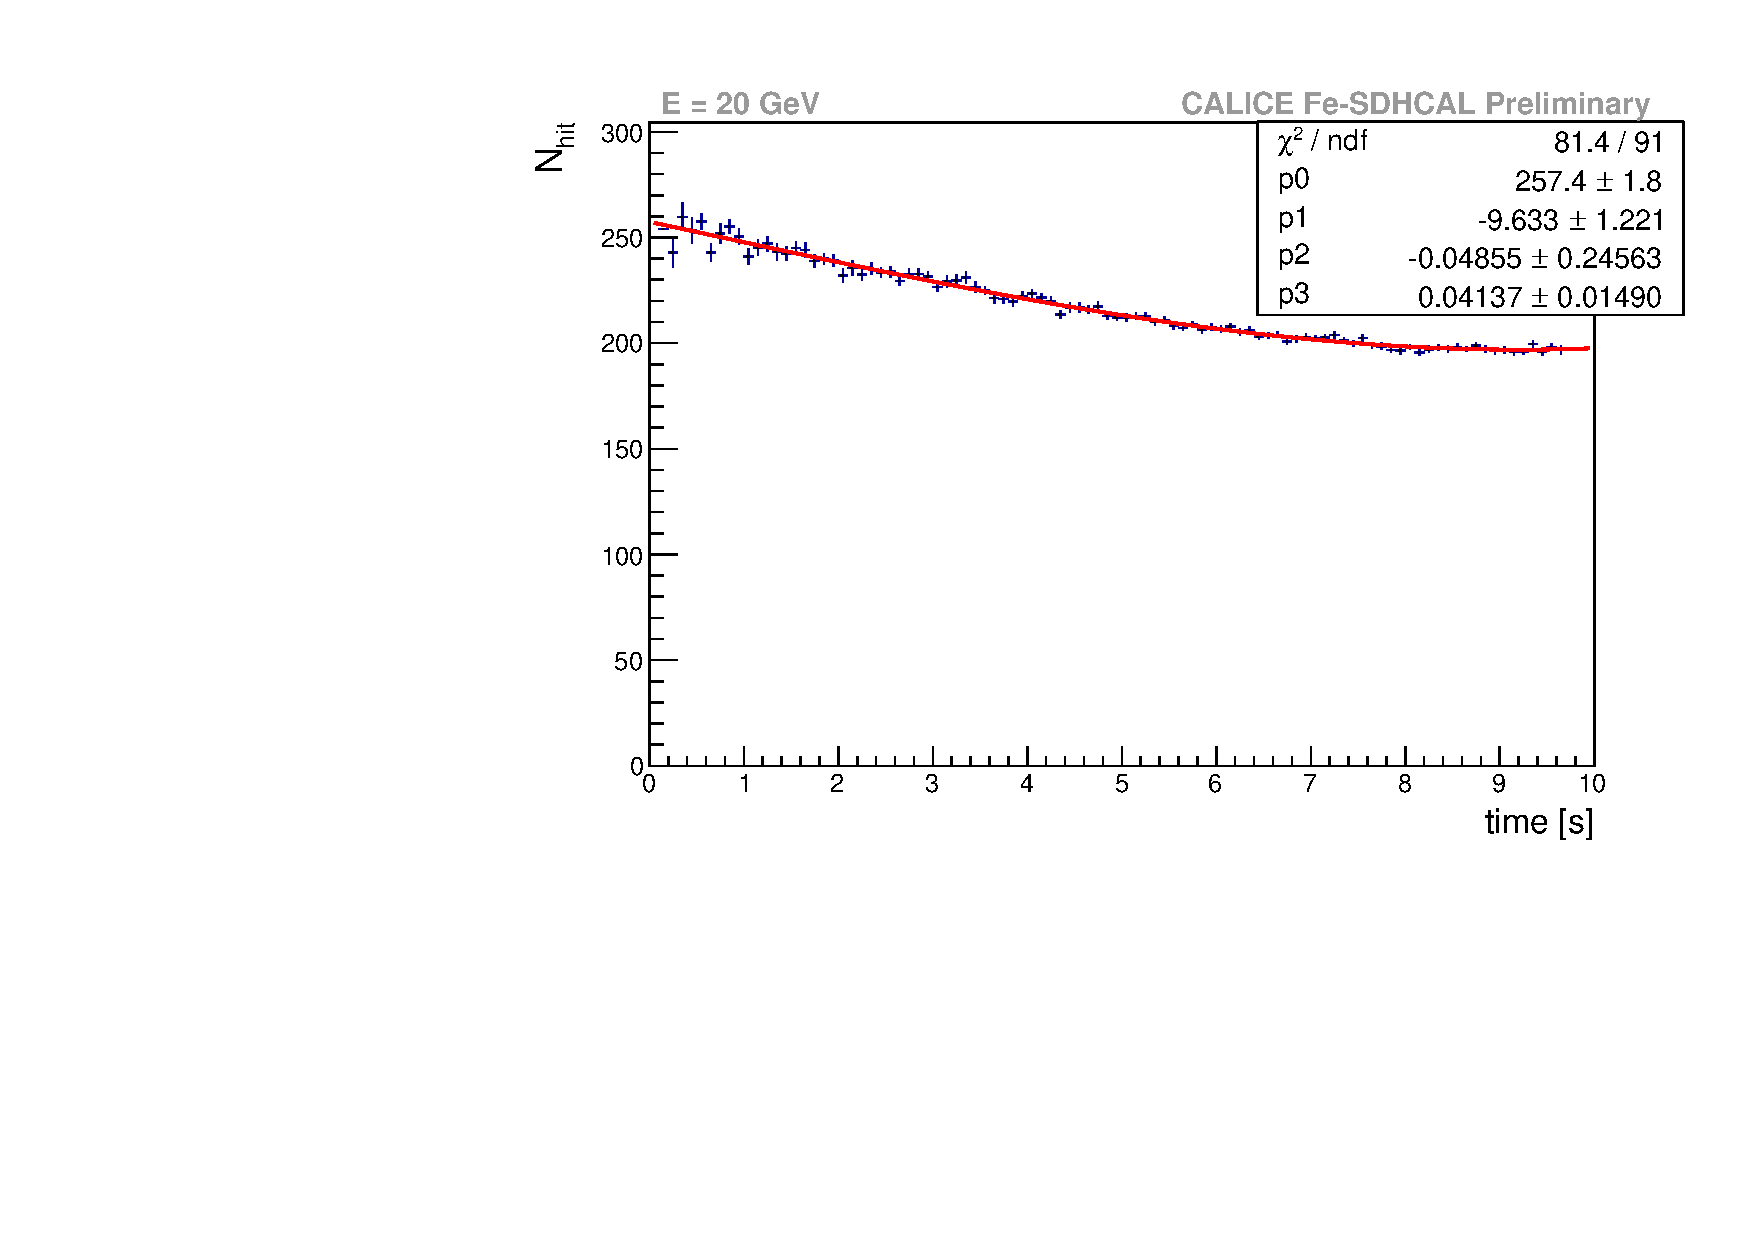
\includegraphics[width=.7\textwidth]{SDHCAL/figs/timeFit.pdf}
    \caption{Correction en fonction du temps.!! Figure avec électrons!!}
    \label{fig:time_correction}
  \end{center}
\end{figure}

\subsection{Reconstruction de l'énergie des pions}
\begin{figure}[!h]
  \begin{center}
    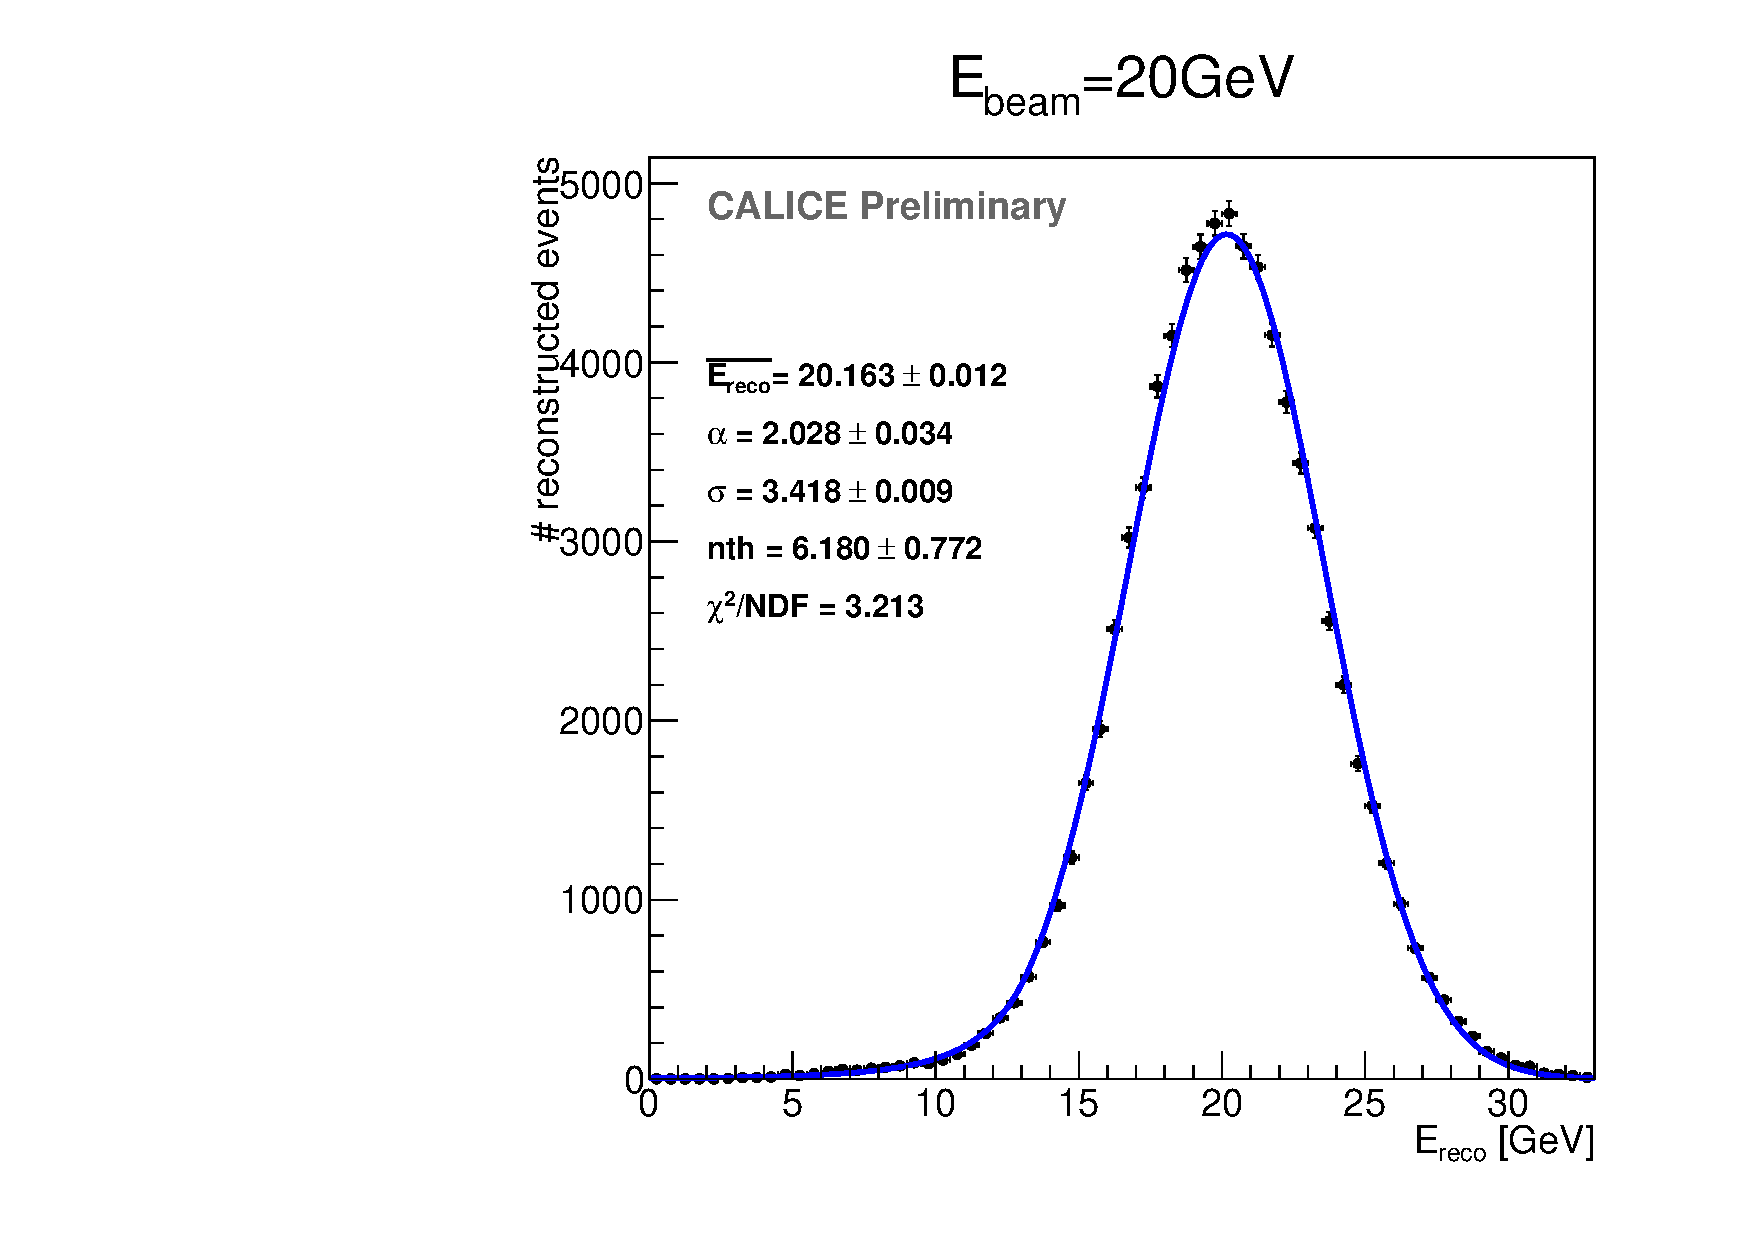
\includegraphics[width=.45\textwidth]{SDHCAL/figs/result20GeV.pdf}
    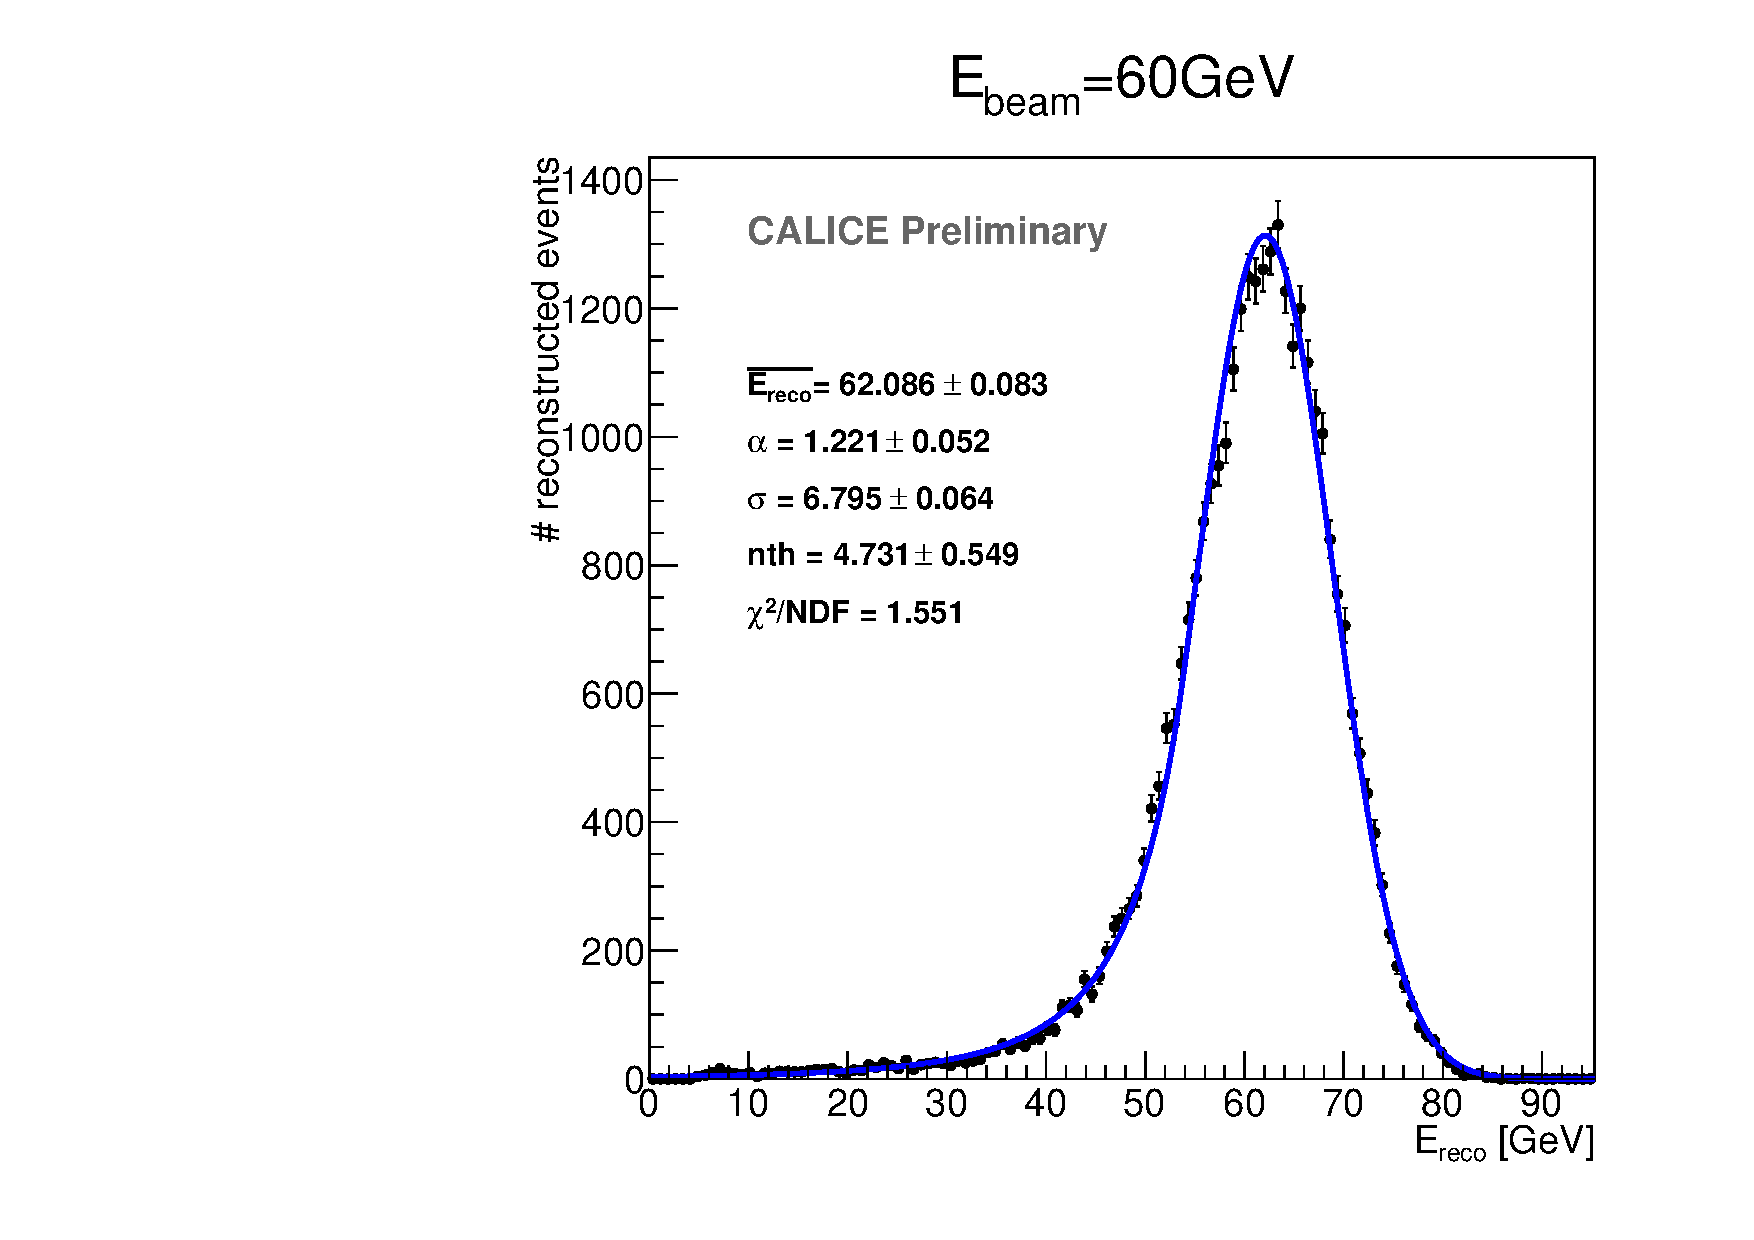
\includegraphics[width=.45\textwidth]{SDHCAL/figs/result60GeV.pdf}
    \caption{Distribution en énergie.}
    \label{fig:energy_dist}
  \end{center}
\end{figure}

\begin{figure}[!h]
  \begin{center}
    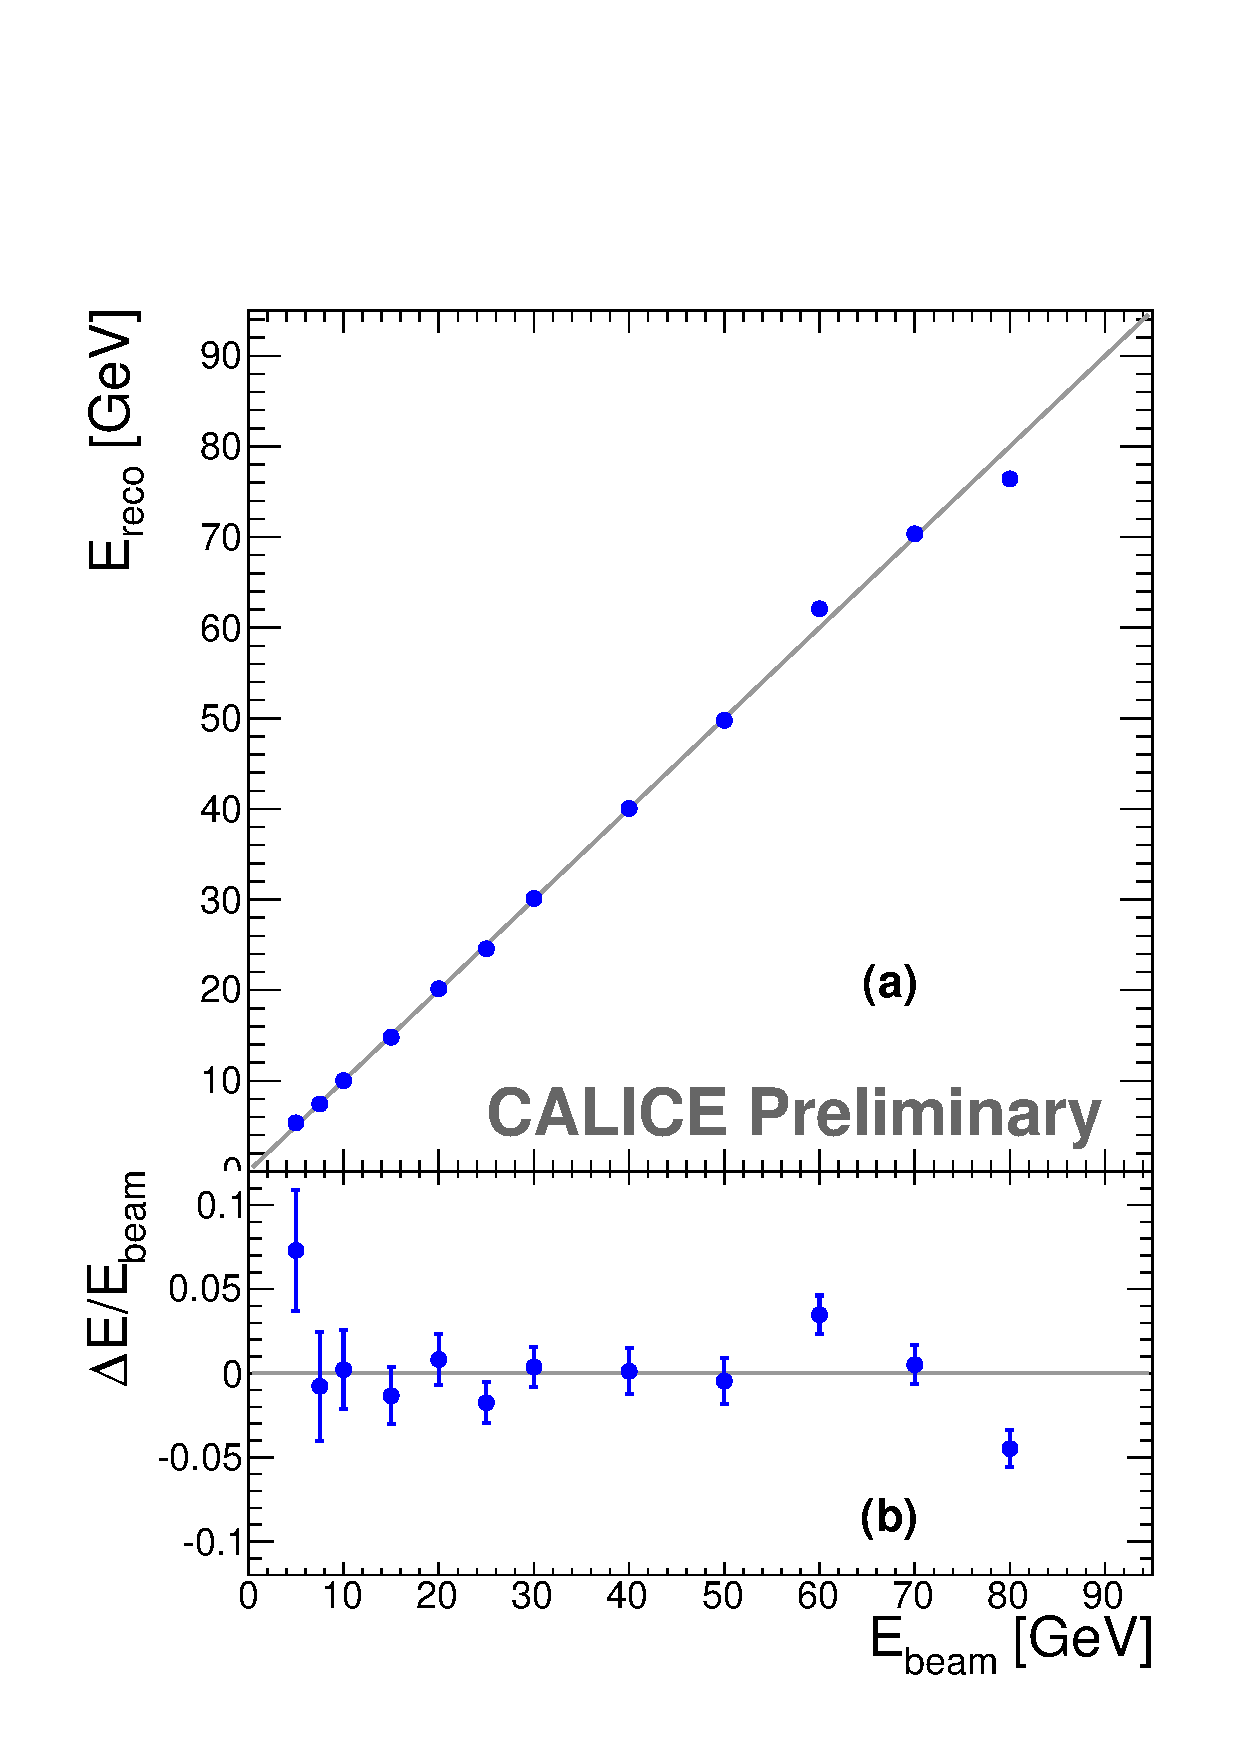
\includegraphics[width=.4\textwidth]{SDHCAL/figs/Energy-Linearity.pdf}
    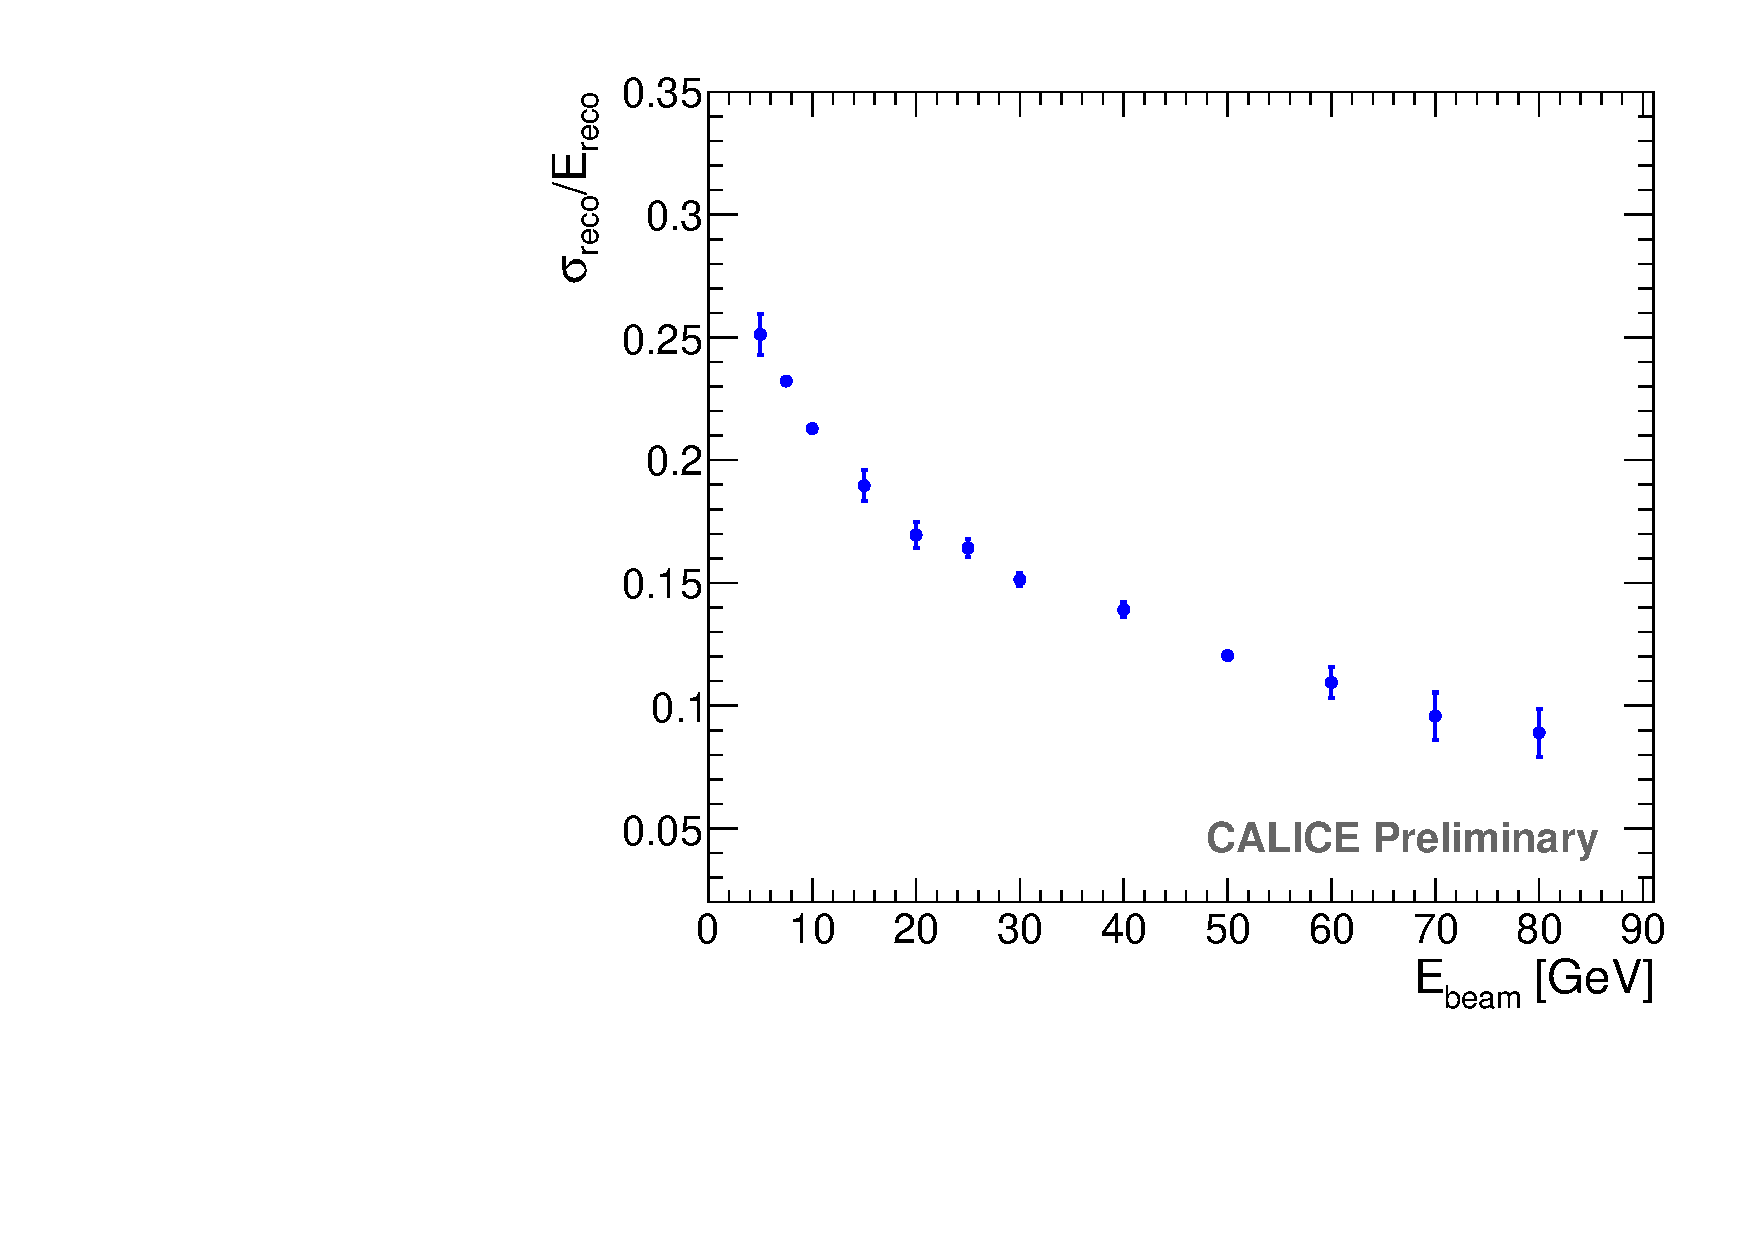
\includegraphics[width=.55\textwidth]{SDHCAL/figs/Energy-Resolution.pdf}
    \caption{Courbe de linéarité et résolution.}
    \label{fig:energy_lin-reso}
  \end{center}
\end{figure}

\begin{figure}[!h]
  \begin{center}
    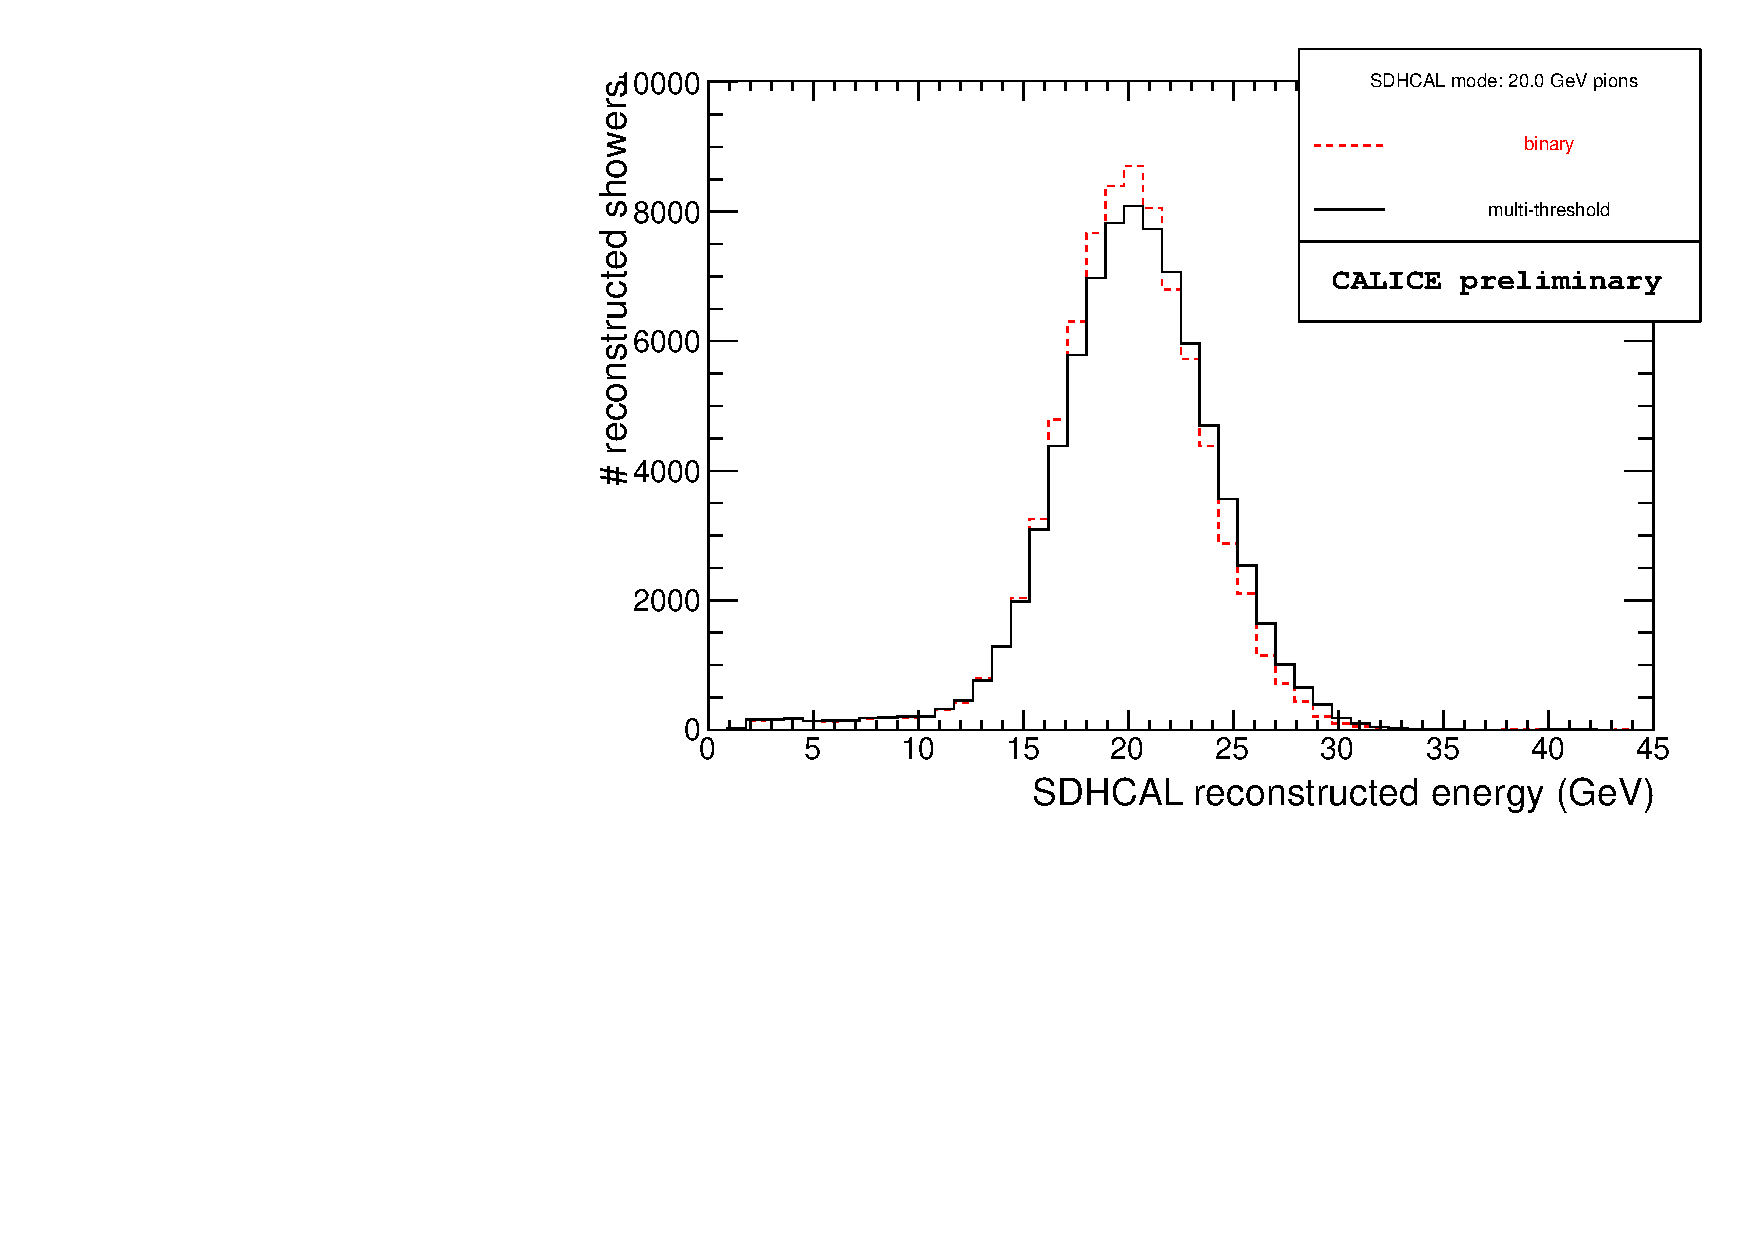
\includegraphics[width=.45\textwidth]{SDHCAL/figs/Pi20GeV_SDHCAL_2modes_overlay.pdf}
    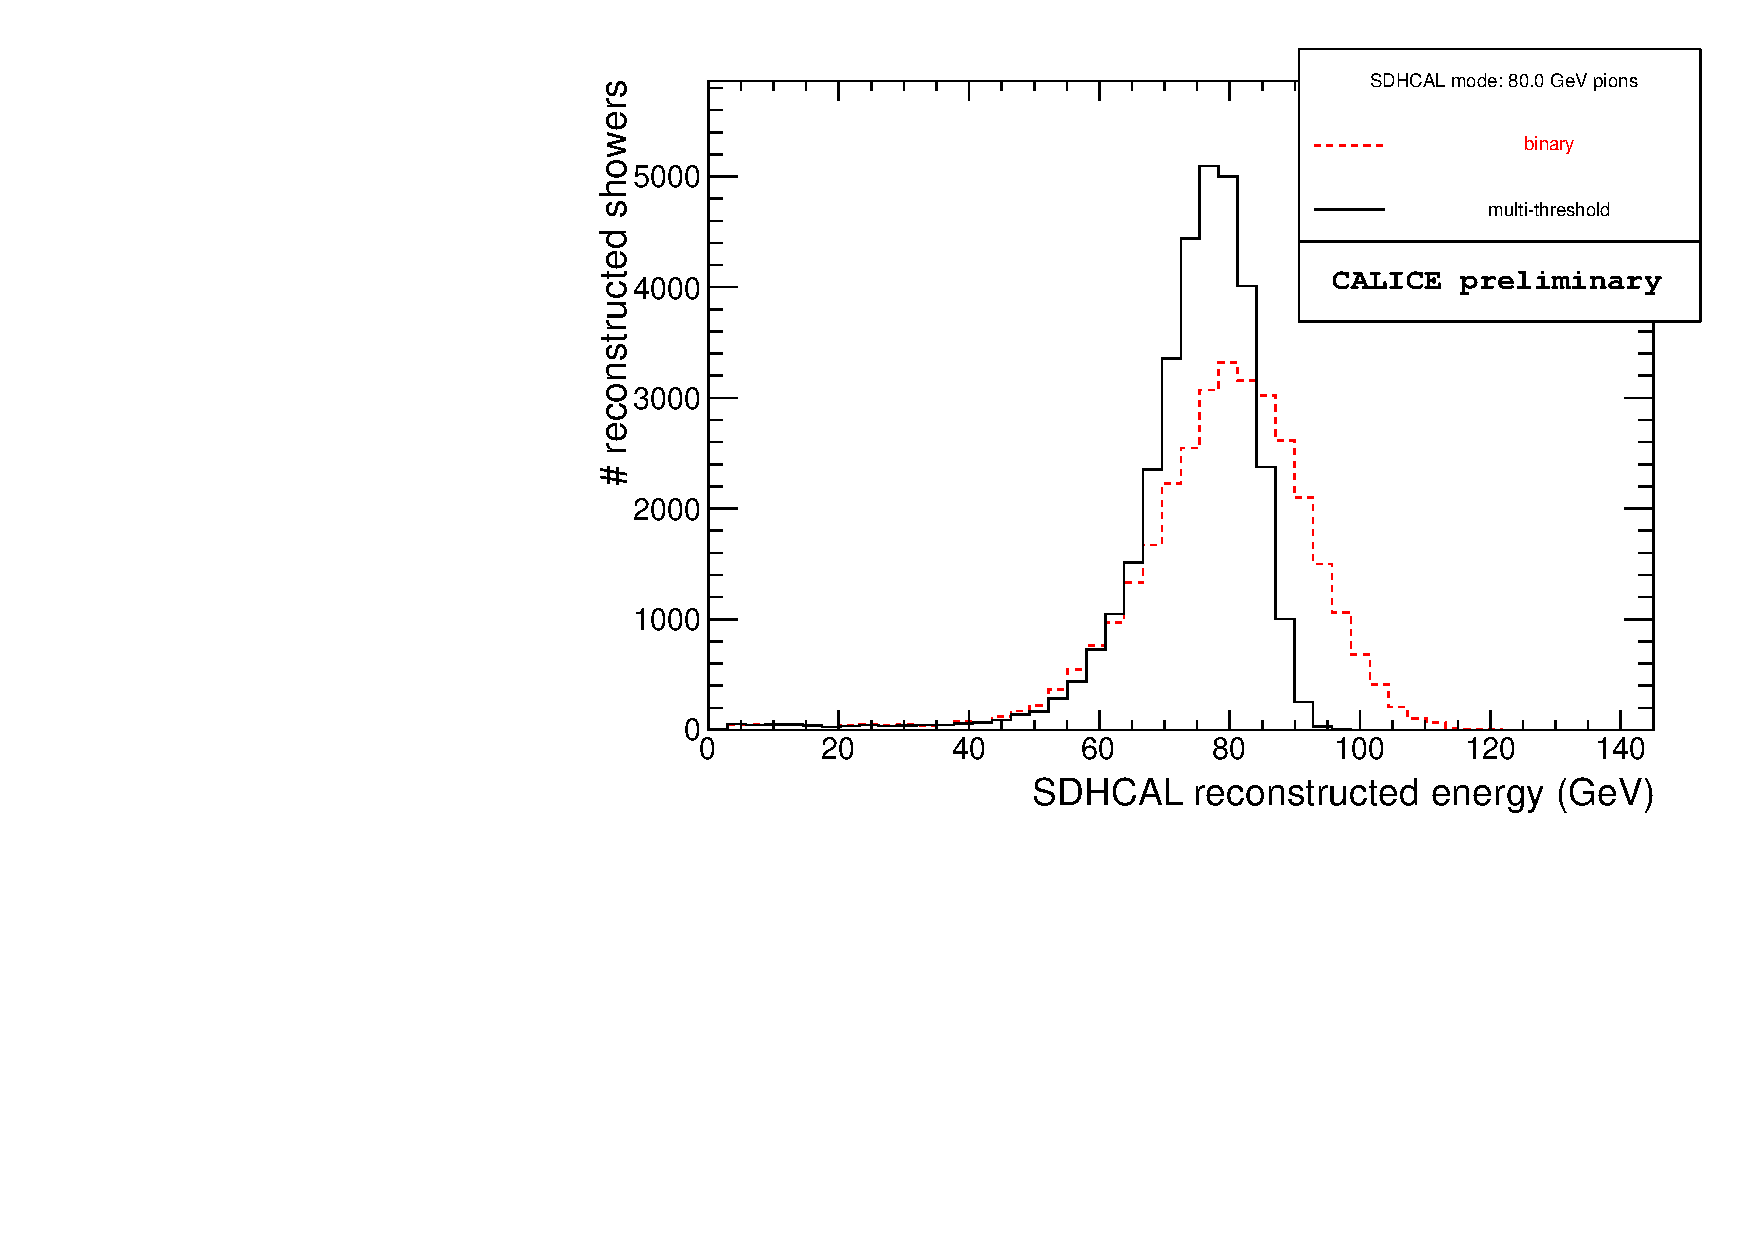
\includegraphics[width=.45\textwidth]{SDHCAL/figs/Pi80GeV_SDHCAL_2modes_overlay.pdf}
    \caption{Comparaison mode binaire et multi-seuils.}
    \label{fig:multi_vs_binary}
  \end{center}
\end{figure}

\begin{figure}[!h]
  \begin{center}
    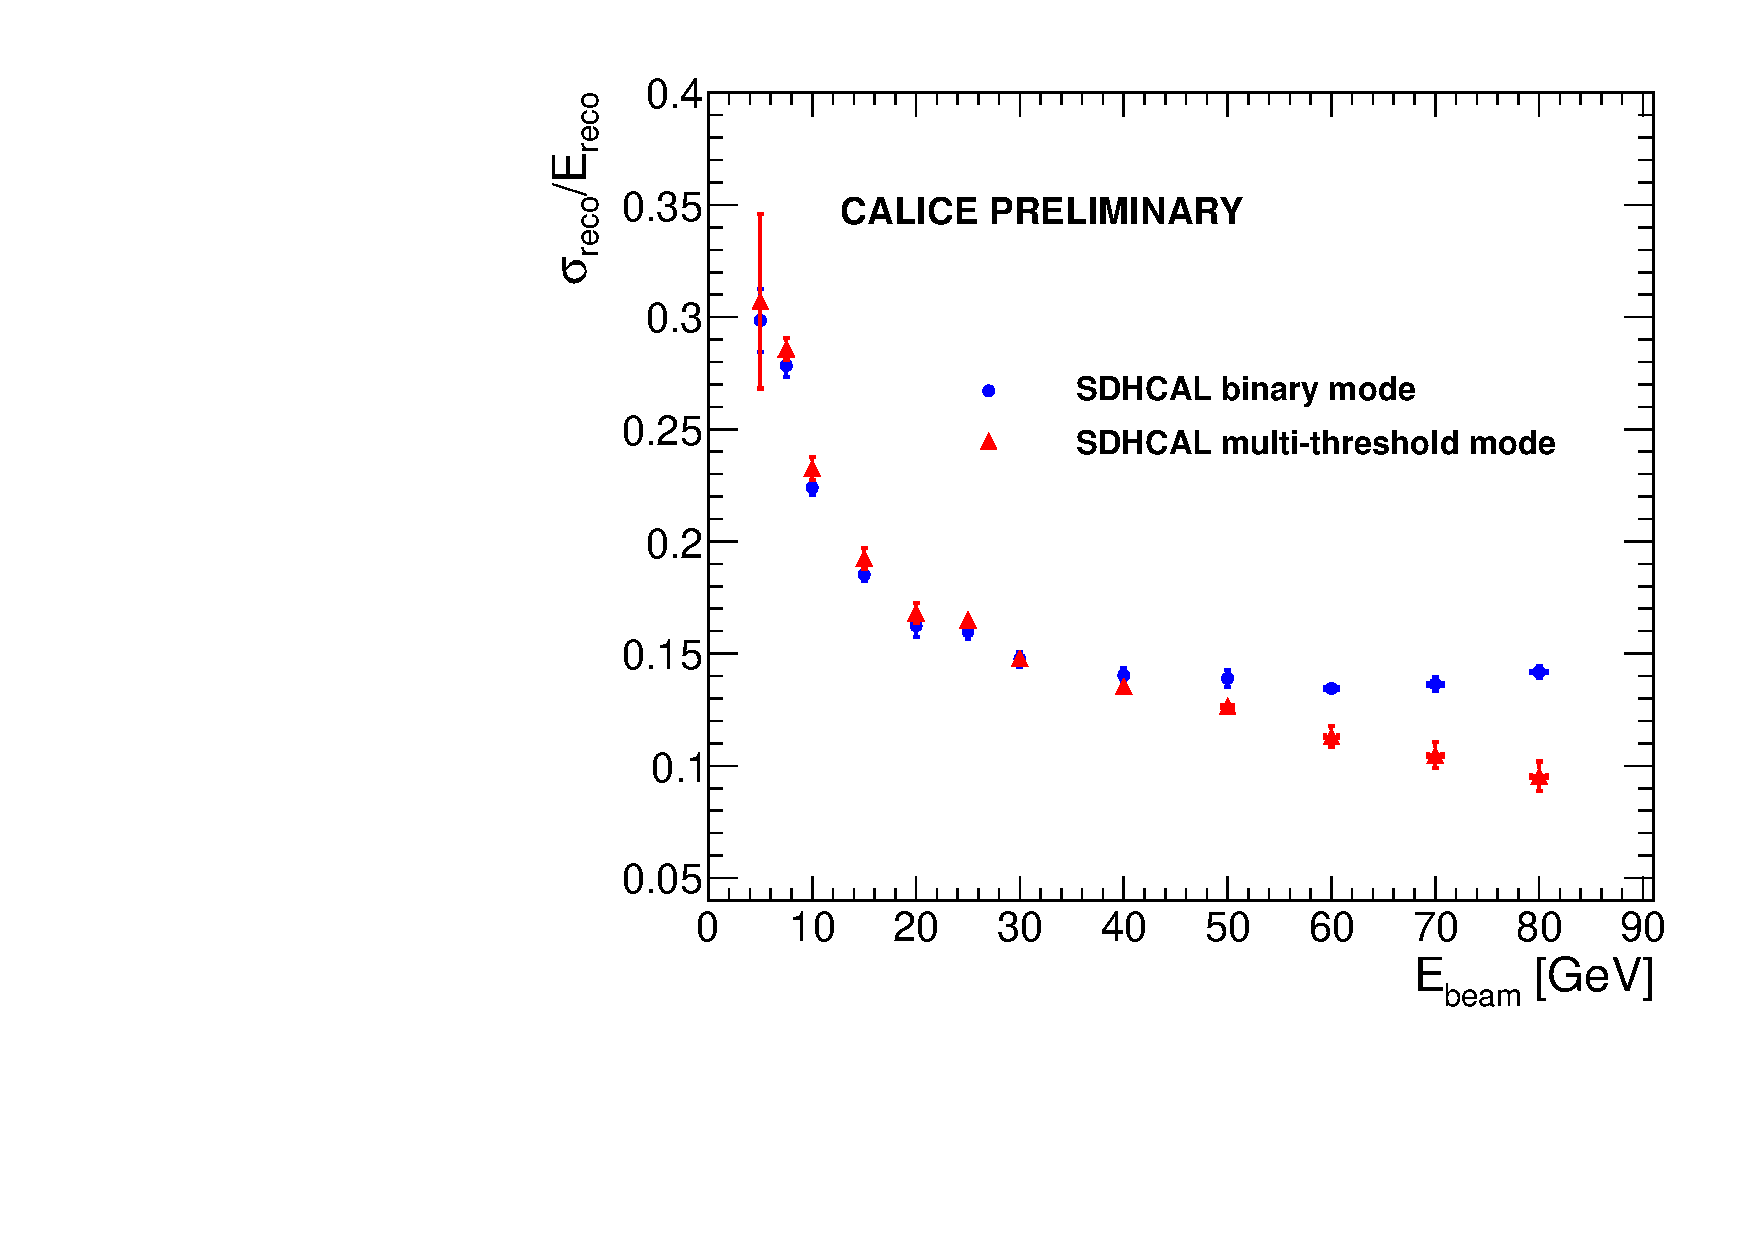
\includegraphics[width=.55\textwidth]{SDHCAL/figs/RESOLUTION.pdf}
    \caption{Résolution en énergie en fonction de l’énergie du faisceau pour le mode binaire et multi-seuils.}
    \label{fig:multi_vs_binary}
  \end{center}
\end{figure}
